\documentclass[10pt]{beamer}

\usetheme{metropolis}
\usepackage{appendixnumberbeamer}

\usepackage{graphicx}
\graphicspath{ {../img/} }

\usepackage{multirow}
\usepackage{booktabs} % Allows the use of \toprule, \midrule and \bottomrule in tables
\newcommand{\tabitem}{~~\llap{\textbullet}~~}
\usepackage[scale=2]{ccicons}

\usepackage{pgfplots}
\usepgfplotslibrary{dateplot}

\usepackage{xspace}
\newcommand{\themename}{\textbf{\textsc{metropolis}}\xspace}

\usepackage{tikz}
\usetikzlibrary{shapes.geometric, arrows, fit, positioning, calc}
\tikzstyle{data} = [rectangle, rounded corners, minimum width=2.5cm, minimum height=0.8cm, text centered, text width=2.5cm, draw=black, fill=blue!30]

\usepackage{relsize}
\tikzset{fontscale/.style = {font=\relsize{#1}}}

\usepackage{color}
\newcommand{\tc}[1]{\textcolor{red}{#1}}

{%
\fboxsep=0pt
\fboxrule=2pt
}%

%----------------------------------------------------------------------------------------
% TITLE PAGE
%----------------------------------------------------------------------------------------
\title[Interface of 3D Reconstruction]{Development and Application of a Description-based Interface for 3D Reconstruction} % The short title appears at the bottom of every slide, the full title is only on the title page

\author{Kai Wu}
\institute[UBC]
{
University of British Columbia \\ % Your institution for the title page
\medskip
kaywu@ece.ubc.ca \\ % Your email address
}
\date{\today}

\begin{document}

\begin{frame}
\maketitle
\end{frame}

\begin{frame}{Table of contents}
  \setbeamertemplate{section in toc}[sections numbered]
  \tableofcontents[hideallsubsections]
\end{frame}

%----------------------------------------------------------------------------------------
% PRESENTATION SLIDES
%----------------------------------------------------------------------------------------

%------------------------------------------------
\section{Introduction}
%------------------------------------------------
\begin{frame}{Motivation: application}

\begin{figure}
\centering
\begin{tabular}{*{3}{p{3.2cm}}}
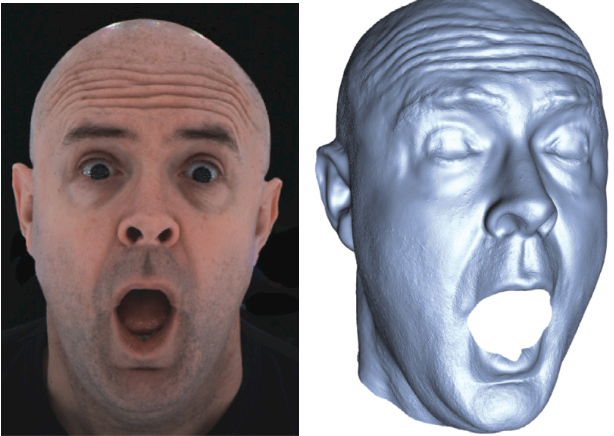
\includegraphics[width=0.3\textwidth]{images/visual_effects.png} &
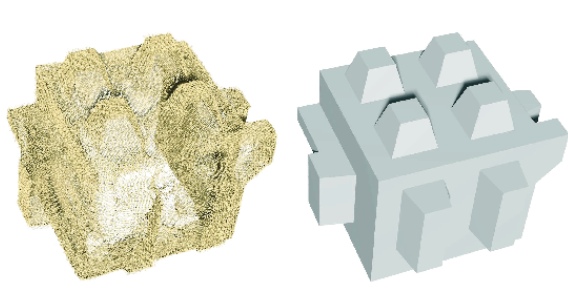
\includegraphics[width=0.3\textwidth]{images/inverse_cad.png} &
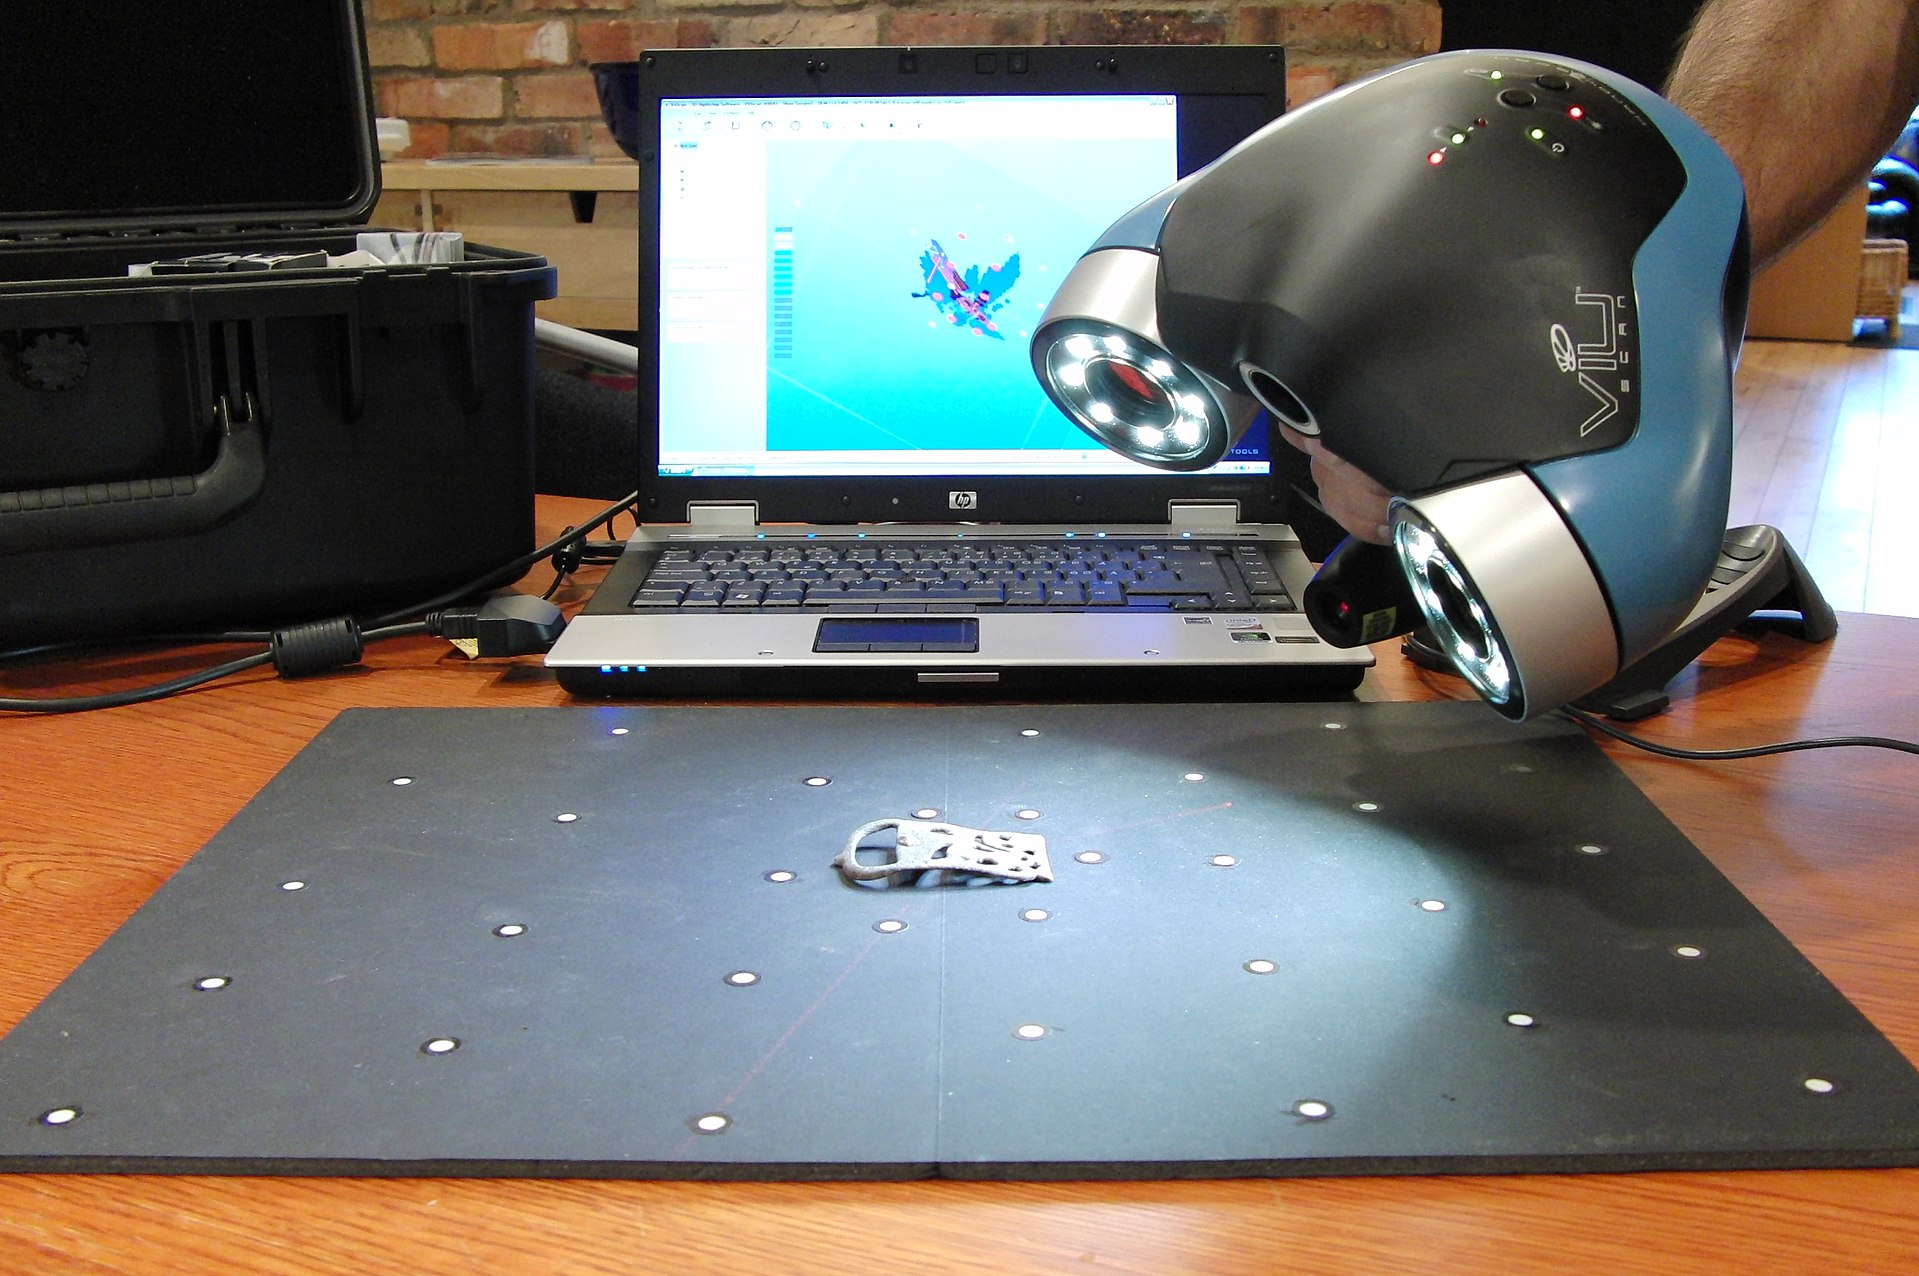
\includegraphics[width=0.3\textwidth]{images/3d_scanner.jpg} \\
Visual effects & Inverse CAD & 3D scanner \\
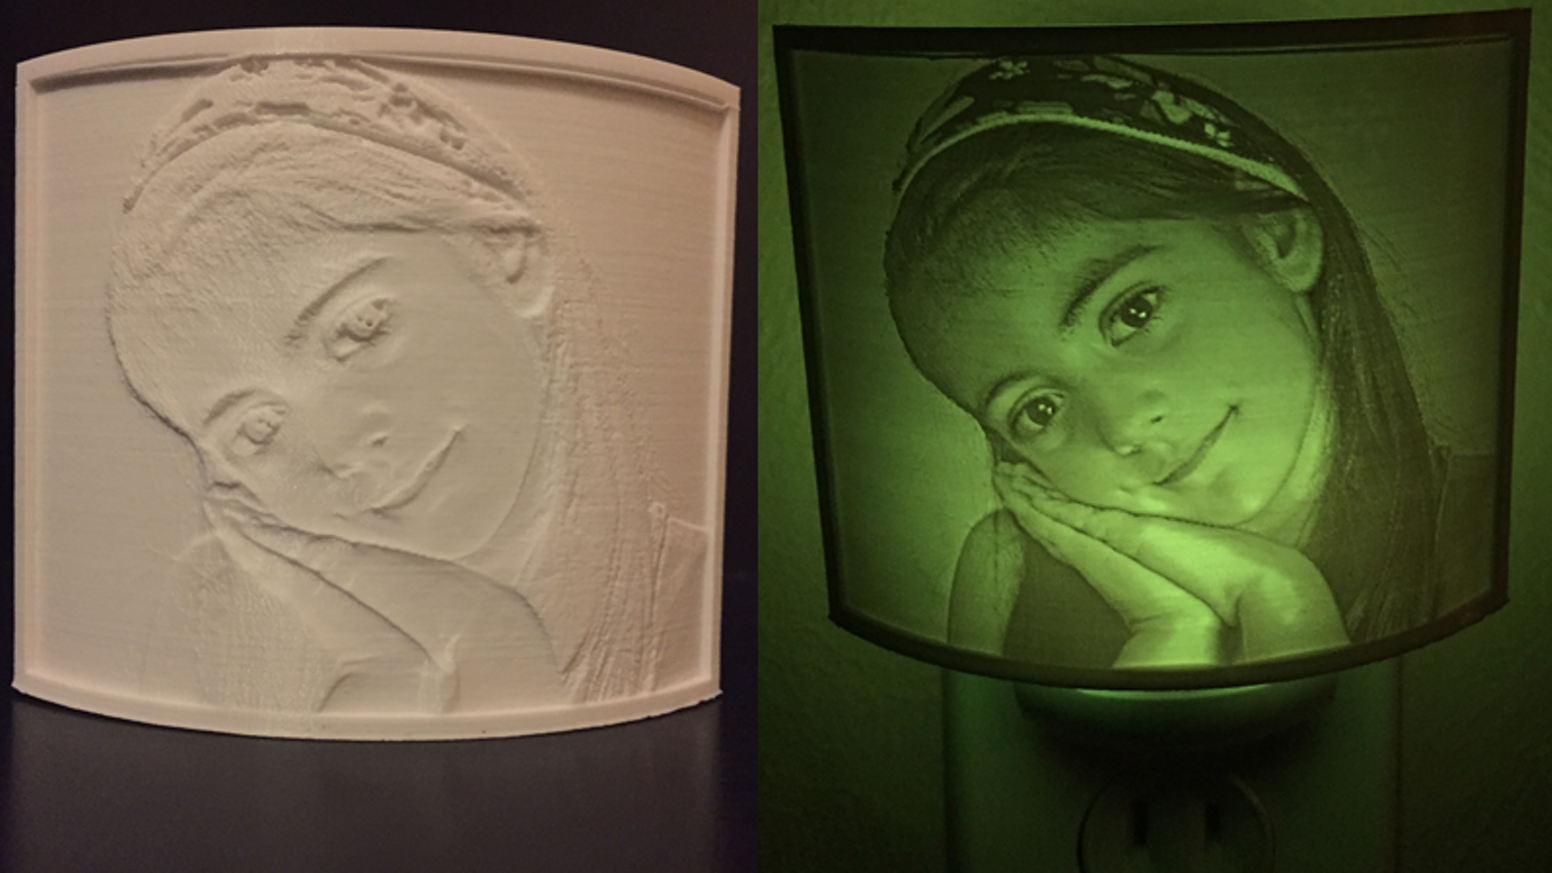
\includegraphics[width=0.3\textwidth]{images/customization.png} & 
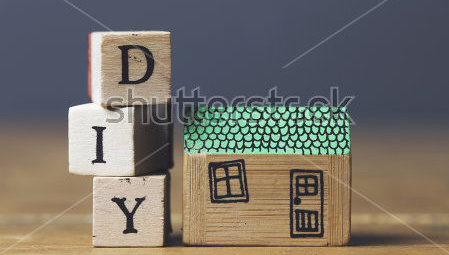
\includegraphics[width=0.3\textwidth]{images/diy_repair_recon.jpg} &
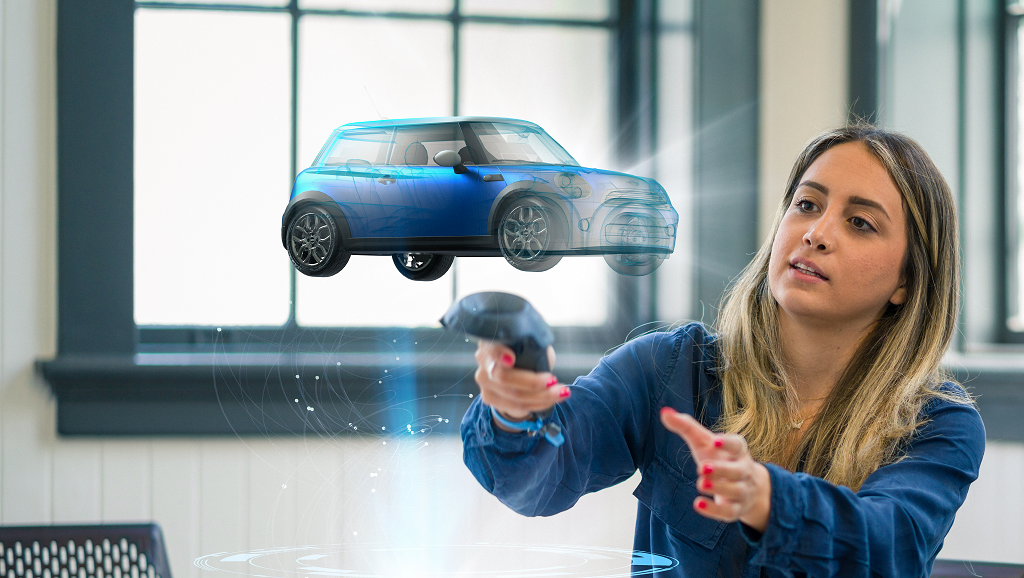
\includegraphics[width=0.3\textwidth]{images/virtual_content.png} \\
Customization & DIY Repair\& Reconstruction & Virtual content creation \\
\end{tabular}
\end{figure}

\end{frame}

%------------------------------------------------
\begin{frame}{Motivation: traditional 3D reconstruction}

\begin{figure}
\centering
\includegraphics[width=0.9\textwidth]{images/3d_recon_traditional_2.pdf}
\end{figure}

\begin{alertblock}{Challenges}
  \begin{itemize}
    \item \textbf{Algorithms}: vision knowledge required;
    \item \textbf{Parameters}: not interpretable, meaningful, or perceptually estimated, vary from algorithm to algorithm.
    \item \textbf{Approach}: \textit{trial-and-error}.
  \end{itemize}
\end{alertblock}

\end{frame}


%------------------------------------------------
\section{Problem Statement} % Research question
%------------------------------------------------
\begin{frame}{Goal}

\begin{table}
\centering
\begin{tabular}{lp{3.5cm}p{4cm}}
& Traditional 3D Recon & Interface for 3D Recon\\
\midrule
Algorithm & vision knowledge & hidden \\
Parameter & algorithm-specific params & a fixed set of params of visual\& geometric properties \\
Approach & multiple trial-and-error & no trial-and-error \\
\end{tabular}
\end{table}

\end{frame}

%------------------------------------------------
\begin{frame}{Contribution}

Development of an interface for 3D reconstruction problem, which hides algorithm details and allows users to describe conditions surrounding the problem. This description can be interpreteded so that an appropriate algorithm is chosen to achieve a successful reconstruction result.

\end{frame}

%------------------------------------------------
% \begin{frame}{Contribution (cont'd)}

% This contribution is significant because:
% \begin{itemize}
% \item Few algorithms can work for a diverse categories of objects. The interface, to some extent, can cover a wider range of object categories by incorporating multiple algorithms.
% \item An description of object problem condition is provided to hide the algorithmic details, thus understanding of the algorithm, or conditions of applying algorithms are not a prerequisite.
% \end{itemize}

% \end{frame}

%------------------------------------------------
\begin{frame}{Overview of thesis/presentation}

\begin{figure}
\centering
\includegraphics[width=\textwidth]{images/thesis_overview.pdf}
\end{figure}

\end{frame}

%------------------------------------------------
\section{Related Work}
%------------------------------------------------
\begin{frame}{Related Work: softwares}

% Some noteable open source general vision libraries and softwares:

\begin{exampleblock}{General vision libraries}
\begin{itemize}
  \item Example: OpenCV, VXL, VLFeat, and so on
  \item Problem: provide APIs for vision routines
\end{itemize}
\end{exampleblock}

\begin{exampleblock}{3D vision softwares}
  \begin{itemize}
    \item Example: PMVS; Bundler, VisualSfM, TheiaSfM; Poisson Recon;
    \item Problem: cater to specific objects, not applicable for textureless surface
  \end{itemize}
\end{exampleblock}

\begin{alertblock}{Challenges}
1. Not that we don't have enough tools, but \textit{when} and \textit{where} to use them. \\
\end{alertblock}

\end{frame}

%------------------------------------------------
\begin{frame}{Related Work: algorithms}

% \begin{exampleblock}{Shape from Stereo}
%   \begin{itemize}
%     \item Example: Multi-View Stereo, Structured Light, laser scanner
%     \item Problem: Texture, reflectance
%   \end{itemize}
% \end{exampleblock}

% \begin{exampleblock}{Shape from Intensity}
%   \begin{itemize}
%     \item Example: Shape from Shading, Photometric Stereo
%     \item Problem: Brightness, geometry
%   \end{itemize}
% \end{exampleblock}

% \begin{exampleblock}{Shape from Silhouette}
%   \begin{itemize}
%     \item Example: Visual Hull, Space Carving
%     \item Problem: Shape, reflectance
%   \end{itemize}
% \end{exampleblock}

\begin{figure}
\begin{tabular}{p{1.6cm}ccp{1.5cm}}
Class & \multicolumn{2}{c}{Method} & Problem \\
\midrule
Shape from Stereo & 
\raisebox{-0.75\height}{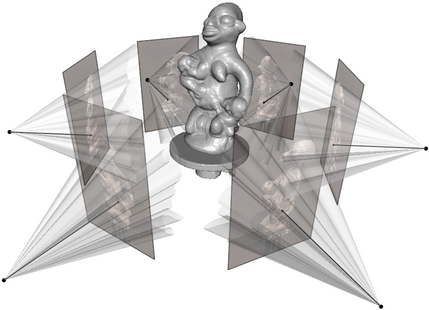
\includegraphics[width=0.2\textwidth]{images/mvs.png}} &
\raisebox{-0.75\height}{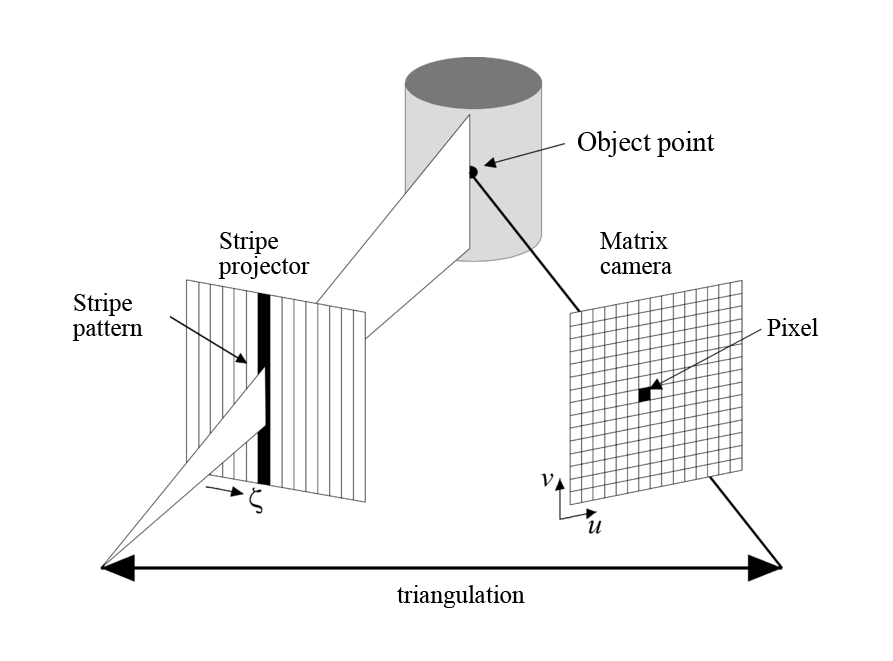
\includegraphics[width=0.2\textwidth]{images/sl.jpg}} &
Texture, Albedo, Specular \\
Shape from Intensity & 
\raisebox{-.75\height}{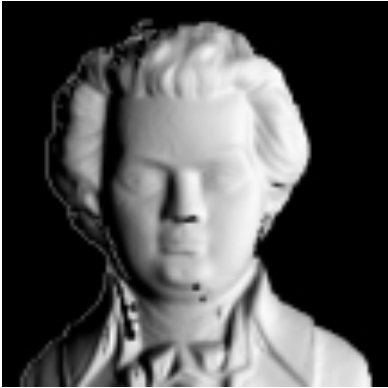
\includegraphics[width=0.15\textwidth]{images/sfs.png}} &
\raisebox{-.75\height}{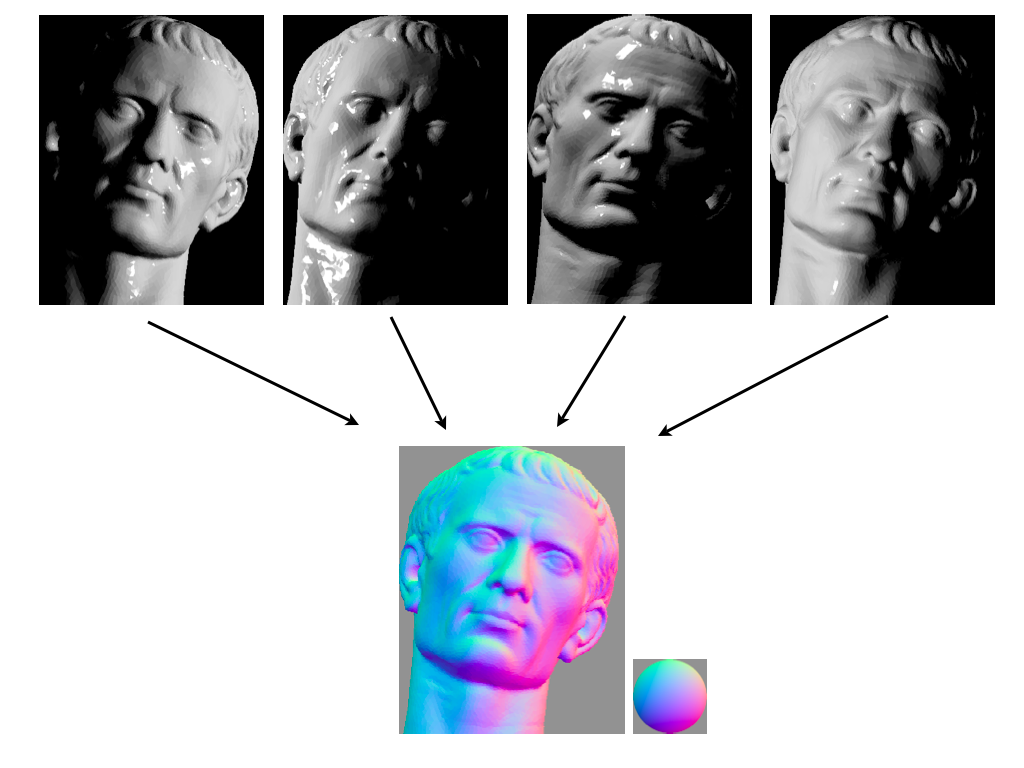
\includegraphics[width=0.2\textwidth]{images/ps.png}} &
Albedo, Specular, Geomtry \\
Shape from Silhouette &
\raisebox{-.75\height}{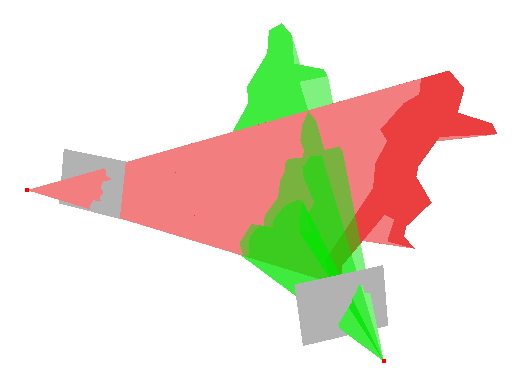
\includegraphics[width=0.2\textwidth]{images/vh.jpg}} &
\raisebox{-.75\height}{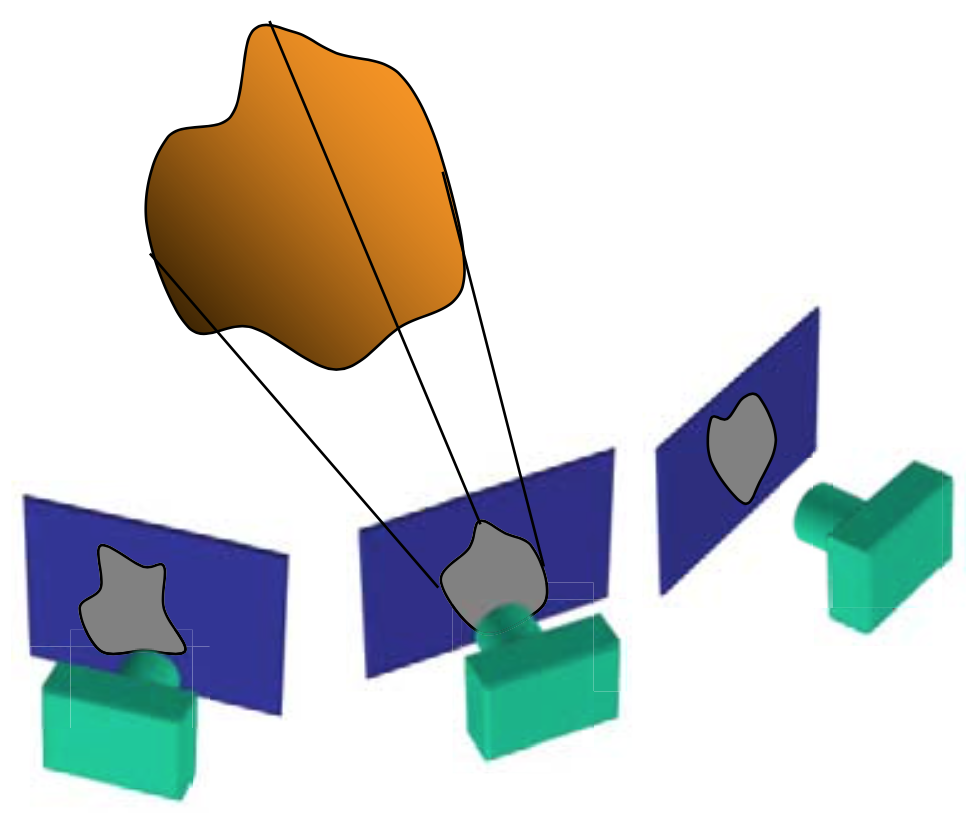
\includegraphics[width=0.2\textwidth]{images/vh_1.png}} &
Geoemtry\\
\end{tabular}
\end{figure}

\begin{alertblock}{Challenges}
1. Few algorithm works for objects with diverse range of properties;\\
2. The range of problem conditions under which an algorithm works is not known a priori.
\end{alertblock}

\end{frame}

%------------------------------------------------
\section{Development of Interface}
%------------------------------------------------
\begin{frame}{Overview of interface}

\begin{exampleblock}{3-layer interface for 3D reconstruction}
\end{exampleblock}

\begin{figure}
\centering
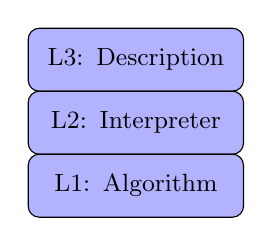
\begin{tikzpicture}[node distance=0.8cm, auto]

\node (desc) [data, font=\small] {L3: Description};
\node (interp) [data, below of=desc, font=\small] {L2: Interpreter};
\node (algo) [data, below of=interp, font=\small] {L1: Algorithm};

\end{tikzpicture}
\end{figure}

\begin{exampleblock}{Description}
  Describe visual and geometric appearance of object
\end{exampleblock}
\begin{exampleblock}{Interpreter}
  1. Translate description into an appropriate algorithm; \\
  2. Mapping: relation between problem space and algorithms.
\end{exampleblock}
\begin{exampleblock}{Algorithm}
  Underlying algorithms across varied categories.
\end{exampleblock}

\end{frame}

%------------------------------------------------
\subsection{Problem Space of 3D Reconstruction}
%------------------------------------------------
\begin{frame}{Problem space}

\begin{exampleblock}{}
% The selection of the properties is based on:
\begin{itemize}
\item Select properties commonly seen in real world;
\item Choose properties that can be addressed by current algorithms.
\end{itemize}
\end{exampleblock}

% \begin{itemize}
% \item \textit{algorithm-centered} approach categorizes algorithms based on algorithm details, as discussed in \textbf{Related Work};
% \item \textit{object-centered} approach categorizes algorithms based on the problem conditions that the algorithm can reliably works under.
% \end{itemize}

\begin{figure}
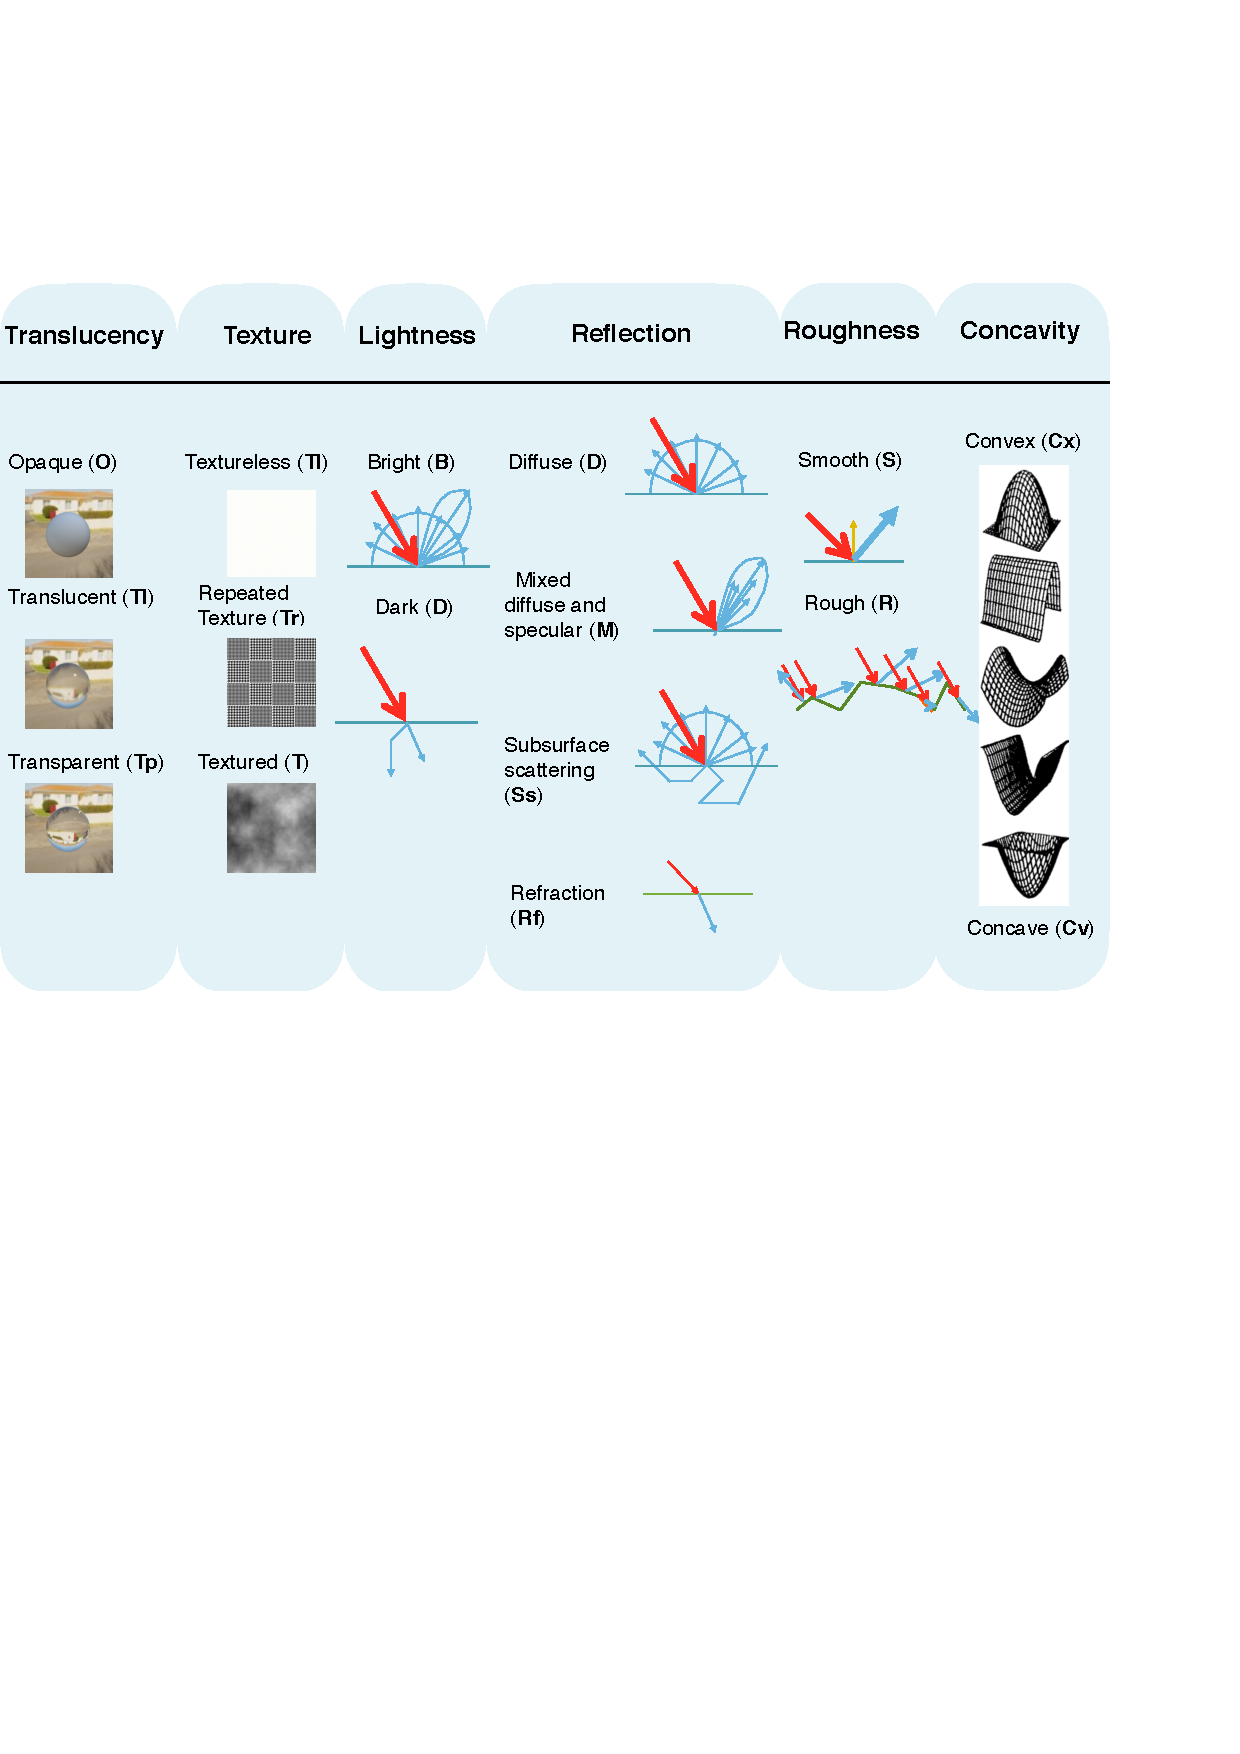
\includegraphics[width=0.8\textwidth]{prob_space/obj_class}
\end{figure}

\end{frame}

%------------------------------------------------
\begin{frame}{Problem space: four problem conditions}

\begin{exampleblock}{Assumptions}

\begin{itemize}
\item \textbf{existence of algorithms}
  \begin{itemize}
  \item translucent, transparent objects need specialized methods;
  \item low surface reflectance, low reflected light.
  \end{itemize}
\item \textbf{local interaction model}
  \begin{itemize}
  \item transmission, refraction, inter-reflection;
  \item severe concavity.
  \end{itemize}
\end{itemize}

\end{exampleblock}

\begin{figure}[h]
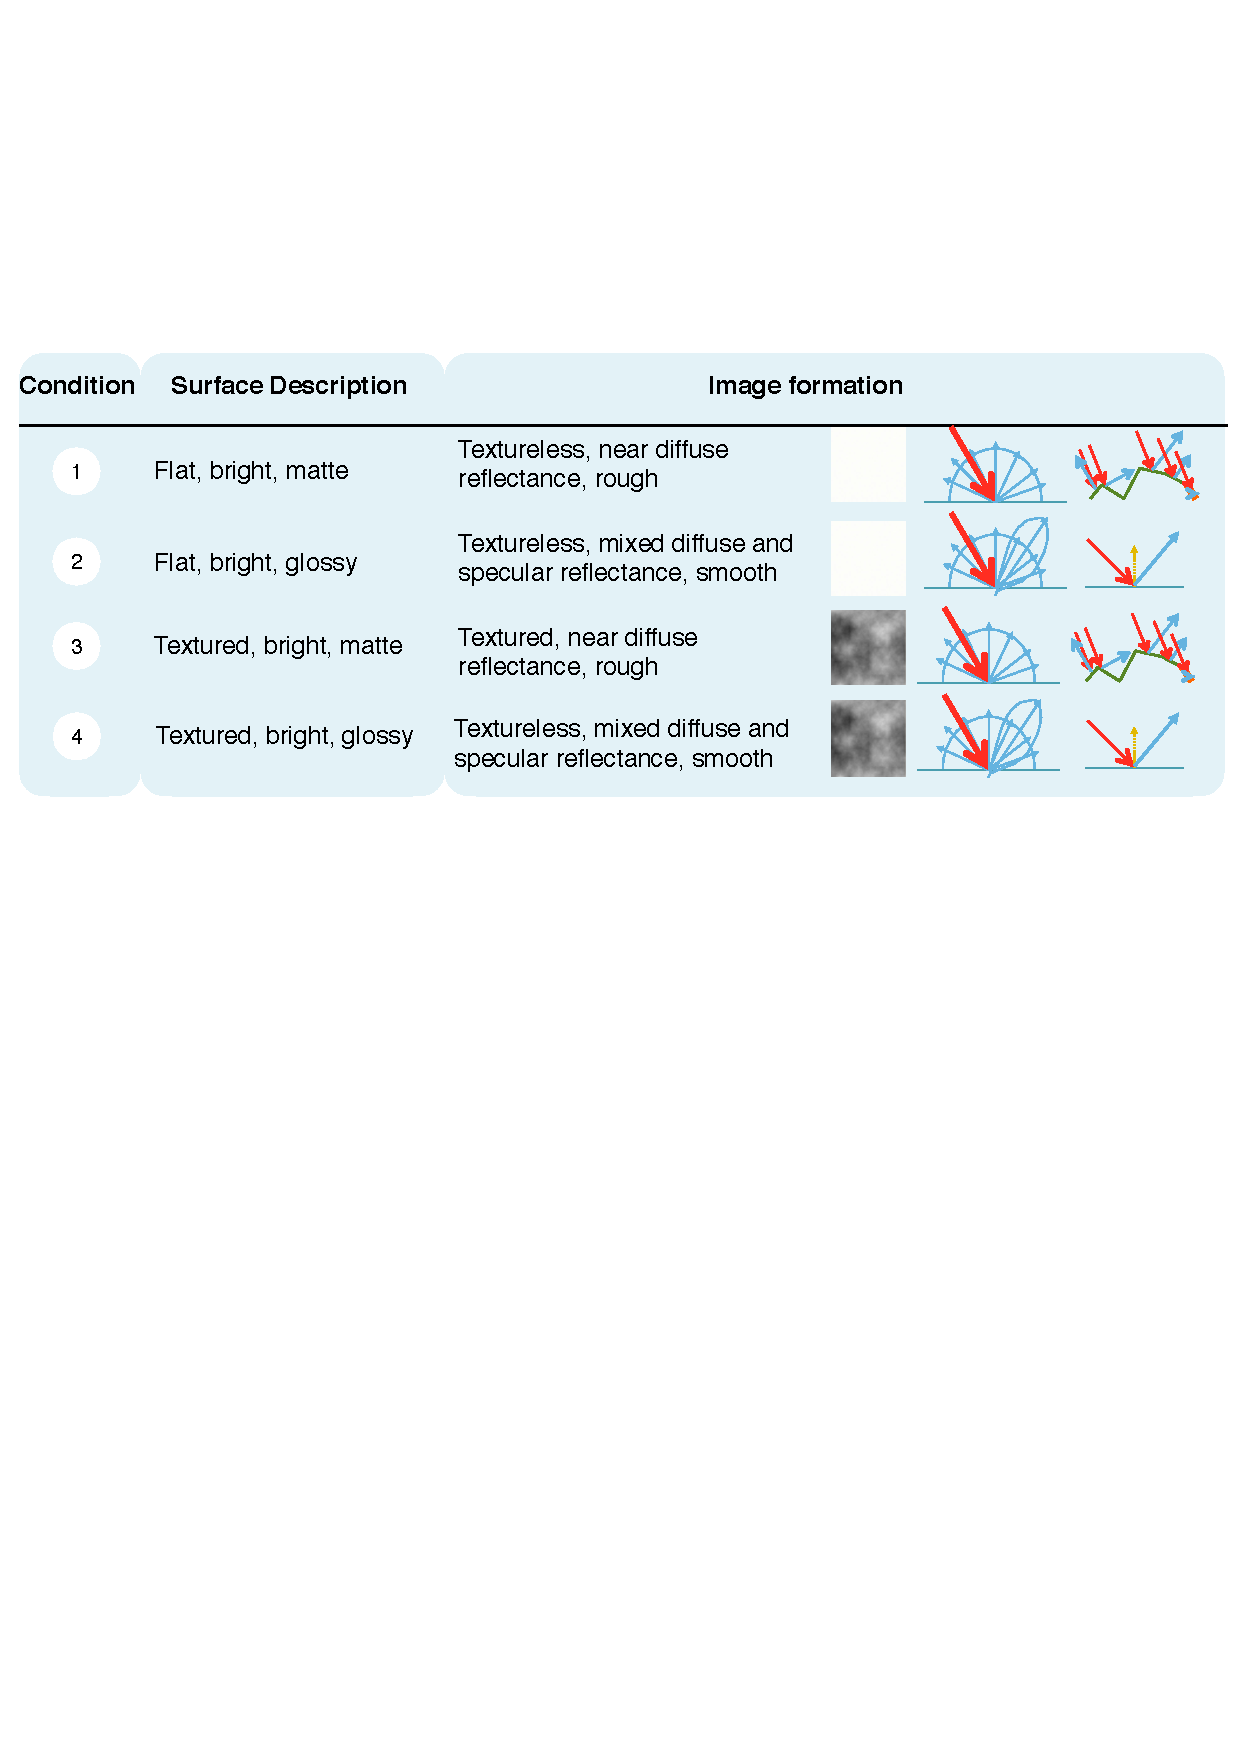
\includegraphics[width=0.8\textwidth]{prob_space/prob_cond}
\end{figure}

\end{frame}

%------------------------------------------------
\subsection{Description of 3D Reconstruction}
%------------------------------------------------
\begin{frame}{Description: model and representations}

\begin{table}
  \centering
  \begin{tabular}{lp{4cm}l}
  \textbf{Model} & \textbf{Representation} & \textbf{Example}\\ \cline{1-3}
  Nature of scene & \textit{Static} \\
  Lighting & \textit{Mixed: ambient, projector, light sources} \\
  Vantage point & \textit{Medium: 10 - 50} \\
  Texture & \textit{Texture randomness} & \raisebox{-.5\height}{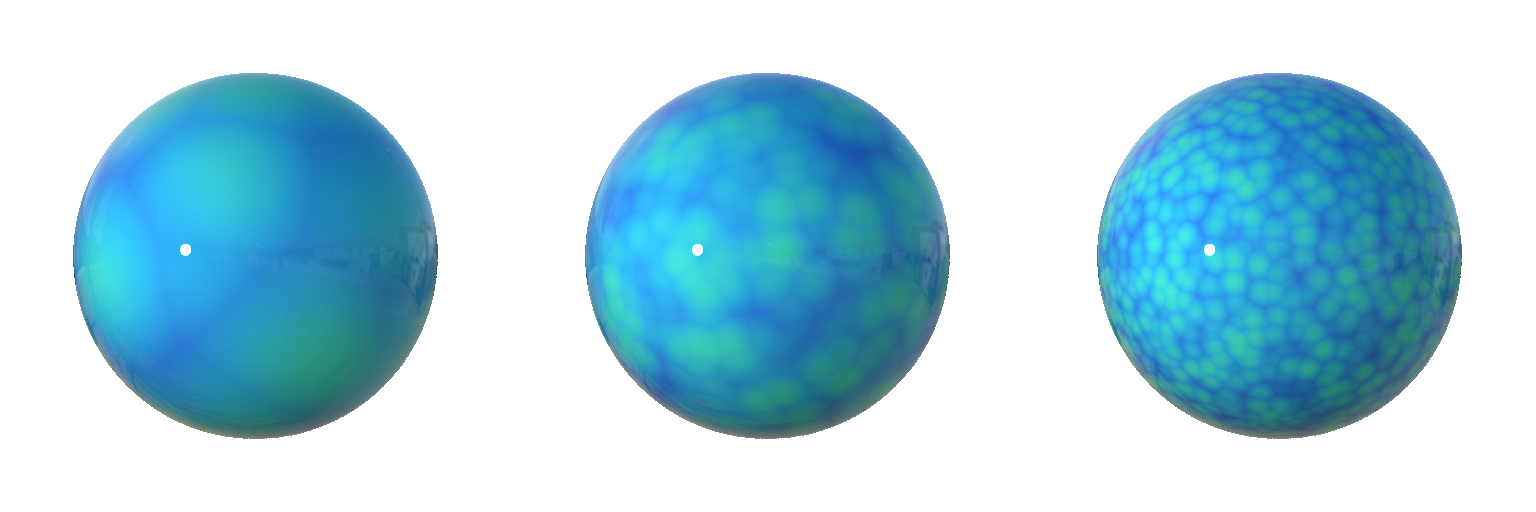
\includegraphics[width=0.3\textwidth]{mapping/setup/tex0}}\\
  Brightness & \textit{Diffuse reflectance} & \raisebox{-.5\height}{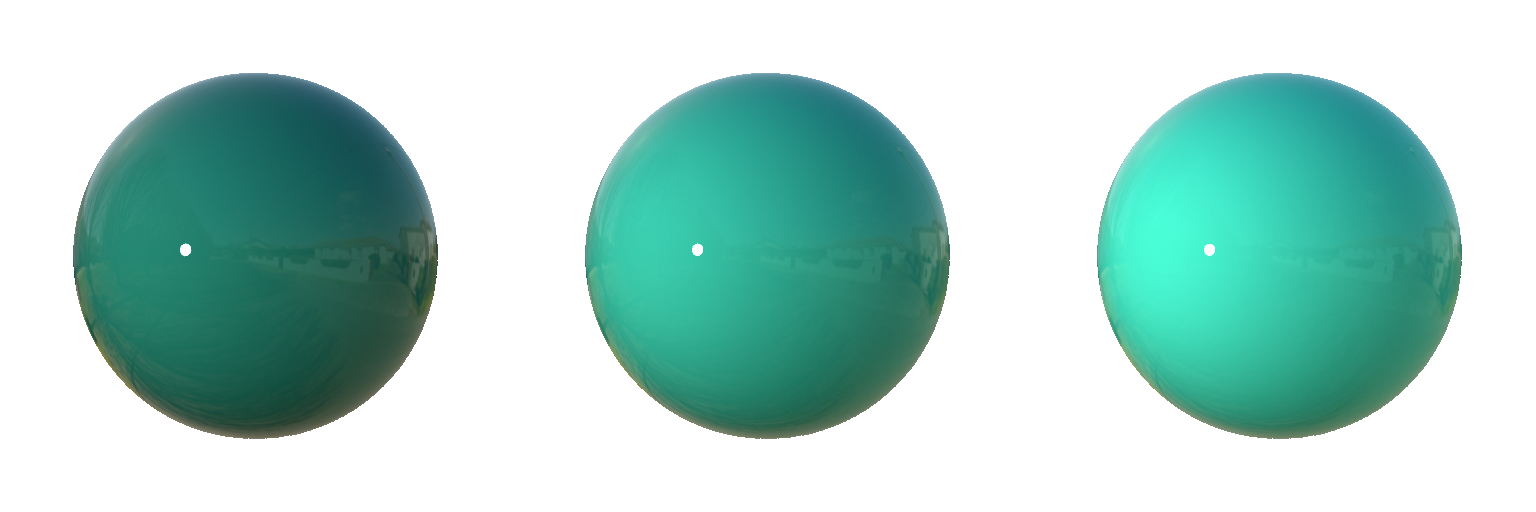
\includegraphics[width=0.3\textwidth]{mapping/setup/alb0}}\\
  Specularity & \textit{Fresnel reflectance} & \raisebox{-.5\height}{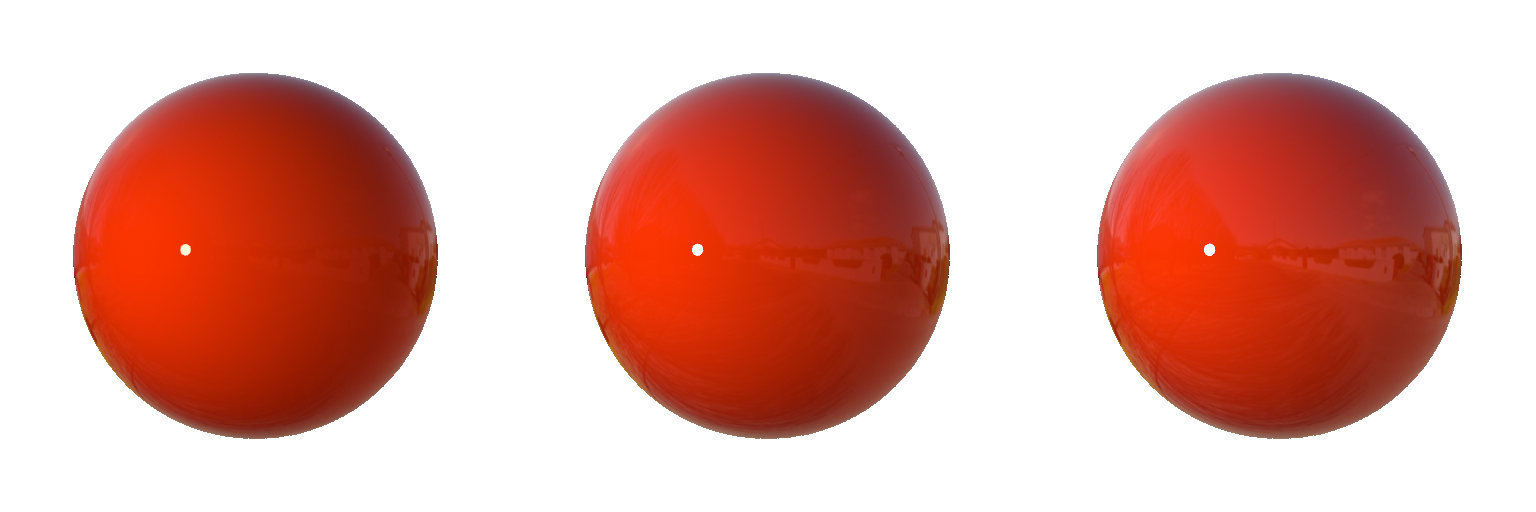
\includegraphics[width=0.3\textwidth]{mapping/setup/spec0}}\\
  Roughness & \textit{Distribution of facet normal} & \raisebox{-.5\height}{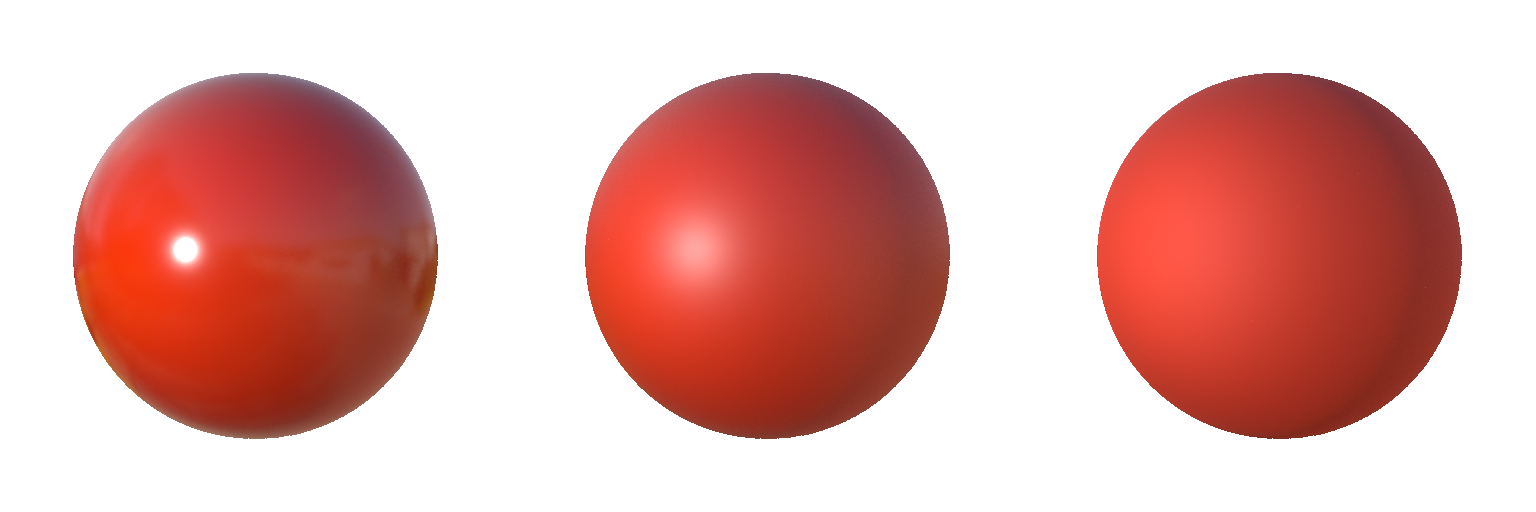
\includegraphics[width=0.3\textwidth]{mapping/setup/rough0}}\\
  % Concavity & \textit{Surface curvature}\\
  \end{tabular}
\end{table}

\end{frame}

%------------------------------------------------
\subsection{Mapping of 3D Reconstruction}
%------------------------------------------------
% \begin{frame}{Mapping: overview}

% % Investigate the problem conditions under which the algorithms can reliably work.
% \begin{figure}
% \centering
% \includegraphics[width=0.9\textwidth]{images/mapping_0.pdf}
% \end{figure}

% \end{frame}

%------------------------------------------------
\begin{frame}{Mapping: dimension reduction}

\begin{figure}
\centering
\includegraphics[width=0.8\textwidth]{images/mapping_1.pdf}
\end{figure}

Reduce problem space dimensionality by discovering properties that have an effect on algorithm performance.

\begin{figure}
\centering
\includegraphics[width=0.5\textwidth]{mapping/eval_prop/mvs_tex_spec}
\end{figure}

\end{frame}

%------------------------------------------------
\begin{frame}{Mapping: mapping construction}

\begin{figure}
\centering
\includegraphics[width=0.8\textwidth]{images/mapping_2.pdf}
\end{figure}

Discover the mapping from problem condition to algorithms.
\begin{figure}
\centering
\includegraphics[width=0.5\textwidth]{mapping/lookup_table/mvs_texture_05}
\end{figure}

\end{frame}

%------------------------------------------------
\section{Application of Interface}
%------------------------------------------------
\begin{frame}{Interpretation: evaluation questions}

\begin{exampleblock}{Evaluation questions}
  1. accurate description $\Rightarrow$ successful result; \\
  2. less accurate description $\Rightarrow$ less successful result;\\
  3. inaccurate description $\Rightarrow$ poor result; \\
\end{exampleblock}

\begin{exampleblock}{Criteria}
  Visual comparison.
\end{exampleblock}

\begin{figure}
\centering
\begin{tabular}{ccc}
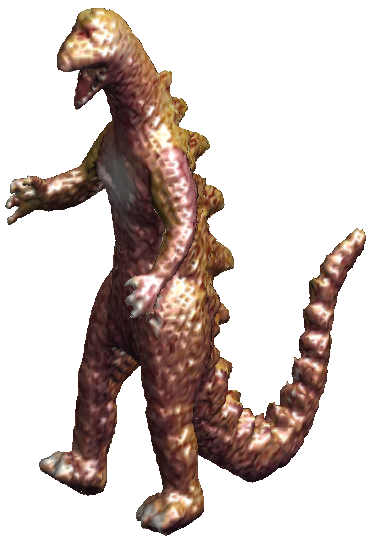
\includegraphics[width=0.2\textwidth]{images/dino.png} &
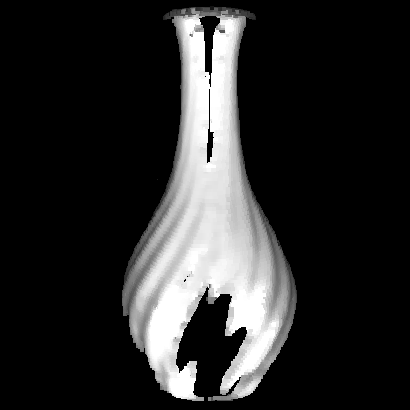
\includegraphics[width=0.2\textwidth]{interp/synth_interp/vase0_sl} &
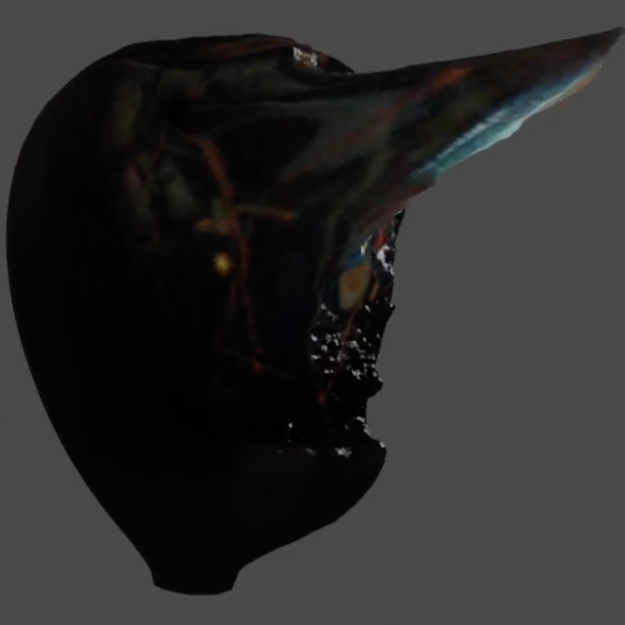
\includegraphics[width=0.2\textwidth]{interp/real_interp/vase/vase_spike} \\
accuracy & completenss & angle diff \\
\end{tabular}
\end{figure}

\end{frame}

%------------------------------------------------
\begin{frame}{Interpretation: dataset creation}

\begin{figure}
\centering
\begin{tabular}{ccc}
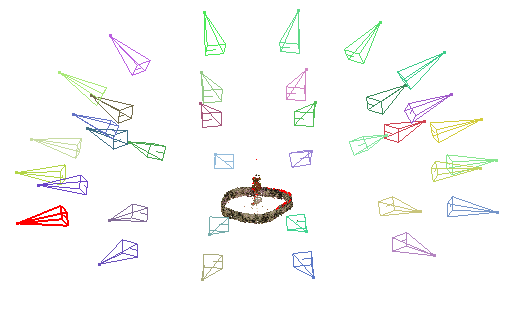
\includegraphics[width=0.3\textwidth]{images/mvs_calib.PNG} &
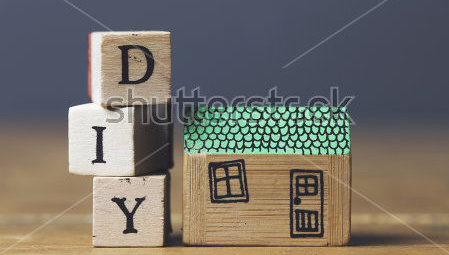
\includegraphics[width=0.3\textwidth]{images/diy_repair_recon.jpg} &
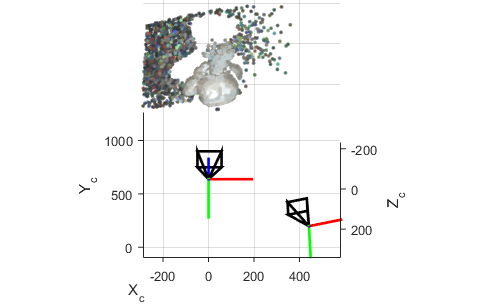
\includegraphics[width=0.3\textwidth]{images/sl_calib.png}\\
MVS\& VH & PS & SL \\
\end{tabular}
\end{figure}

\begin{table}
  \begin{tabular}{p{1cm}p{2cm}p{2.5cm}p{4cm}}
  Alg & Hardware & Config & Calibration \\
  \midrule
  MVS, VH & camera, turntable  & 3 heights, $30^\circ$ baseline angle & focal length from EXIF, extrinsics using SfM \\
  PS & camera, lamp, ref objs & random light position & no radiometric/geometric calibration performed \\
  SL & camera, projector & $10^\circ$ baseline angle & camera-projector calibration using local homography\\
  \end{tabular}
\end{table}

\end{frame}

%------------------------------------------------
\begin{frame}{Interpretation: dataset}

Objects meet the requirements of the four problem conditions.

\begin{figure}[!htbp]
\centering
\begin{tabular}{p{0.4cm}*{4}{c}} % p{1.5cm}
Cond & 1 & 2 & 3 & 4\\
\midrule
\multirow{2}{*}{\rotatebox[origin=c]{90}{Object}} & 
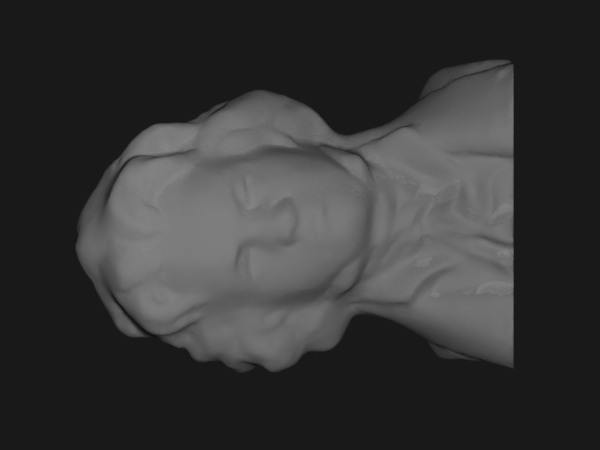
\includegraphics[width=0.15\textwidth]{interp/synth_data/bust} &
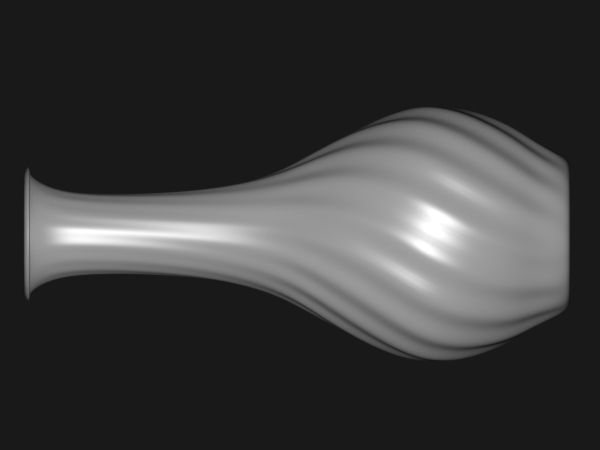
\includegraphics[width=0.15\textwidth]{interp/synth_data/vase0} &
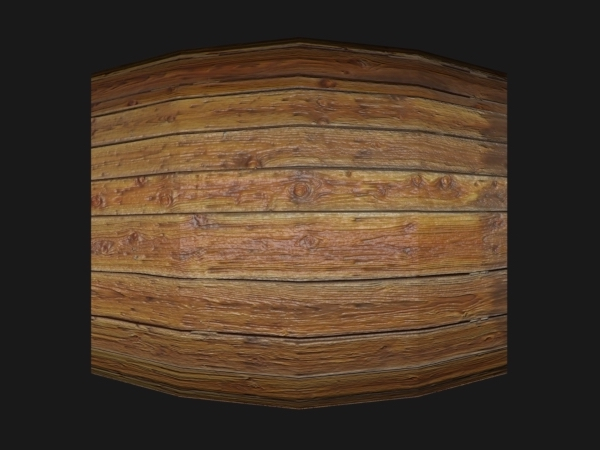
\includegraphics[width=0.15\textwidth]{interp/synth_data/barrel} &
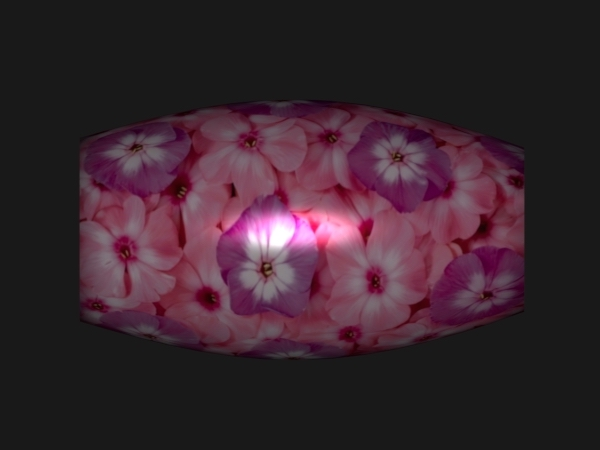
\includegraphics[width=0.15\textwidth]{interp/synth_data/vase1}\\
& 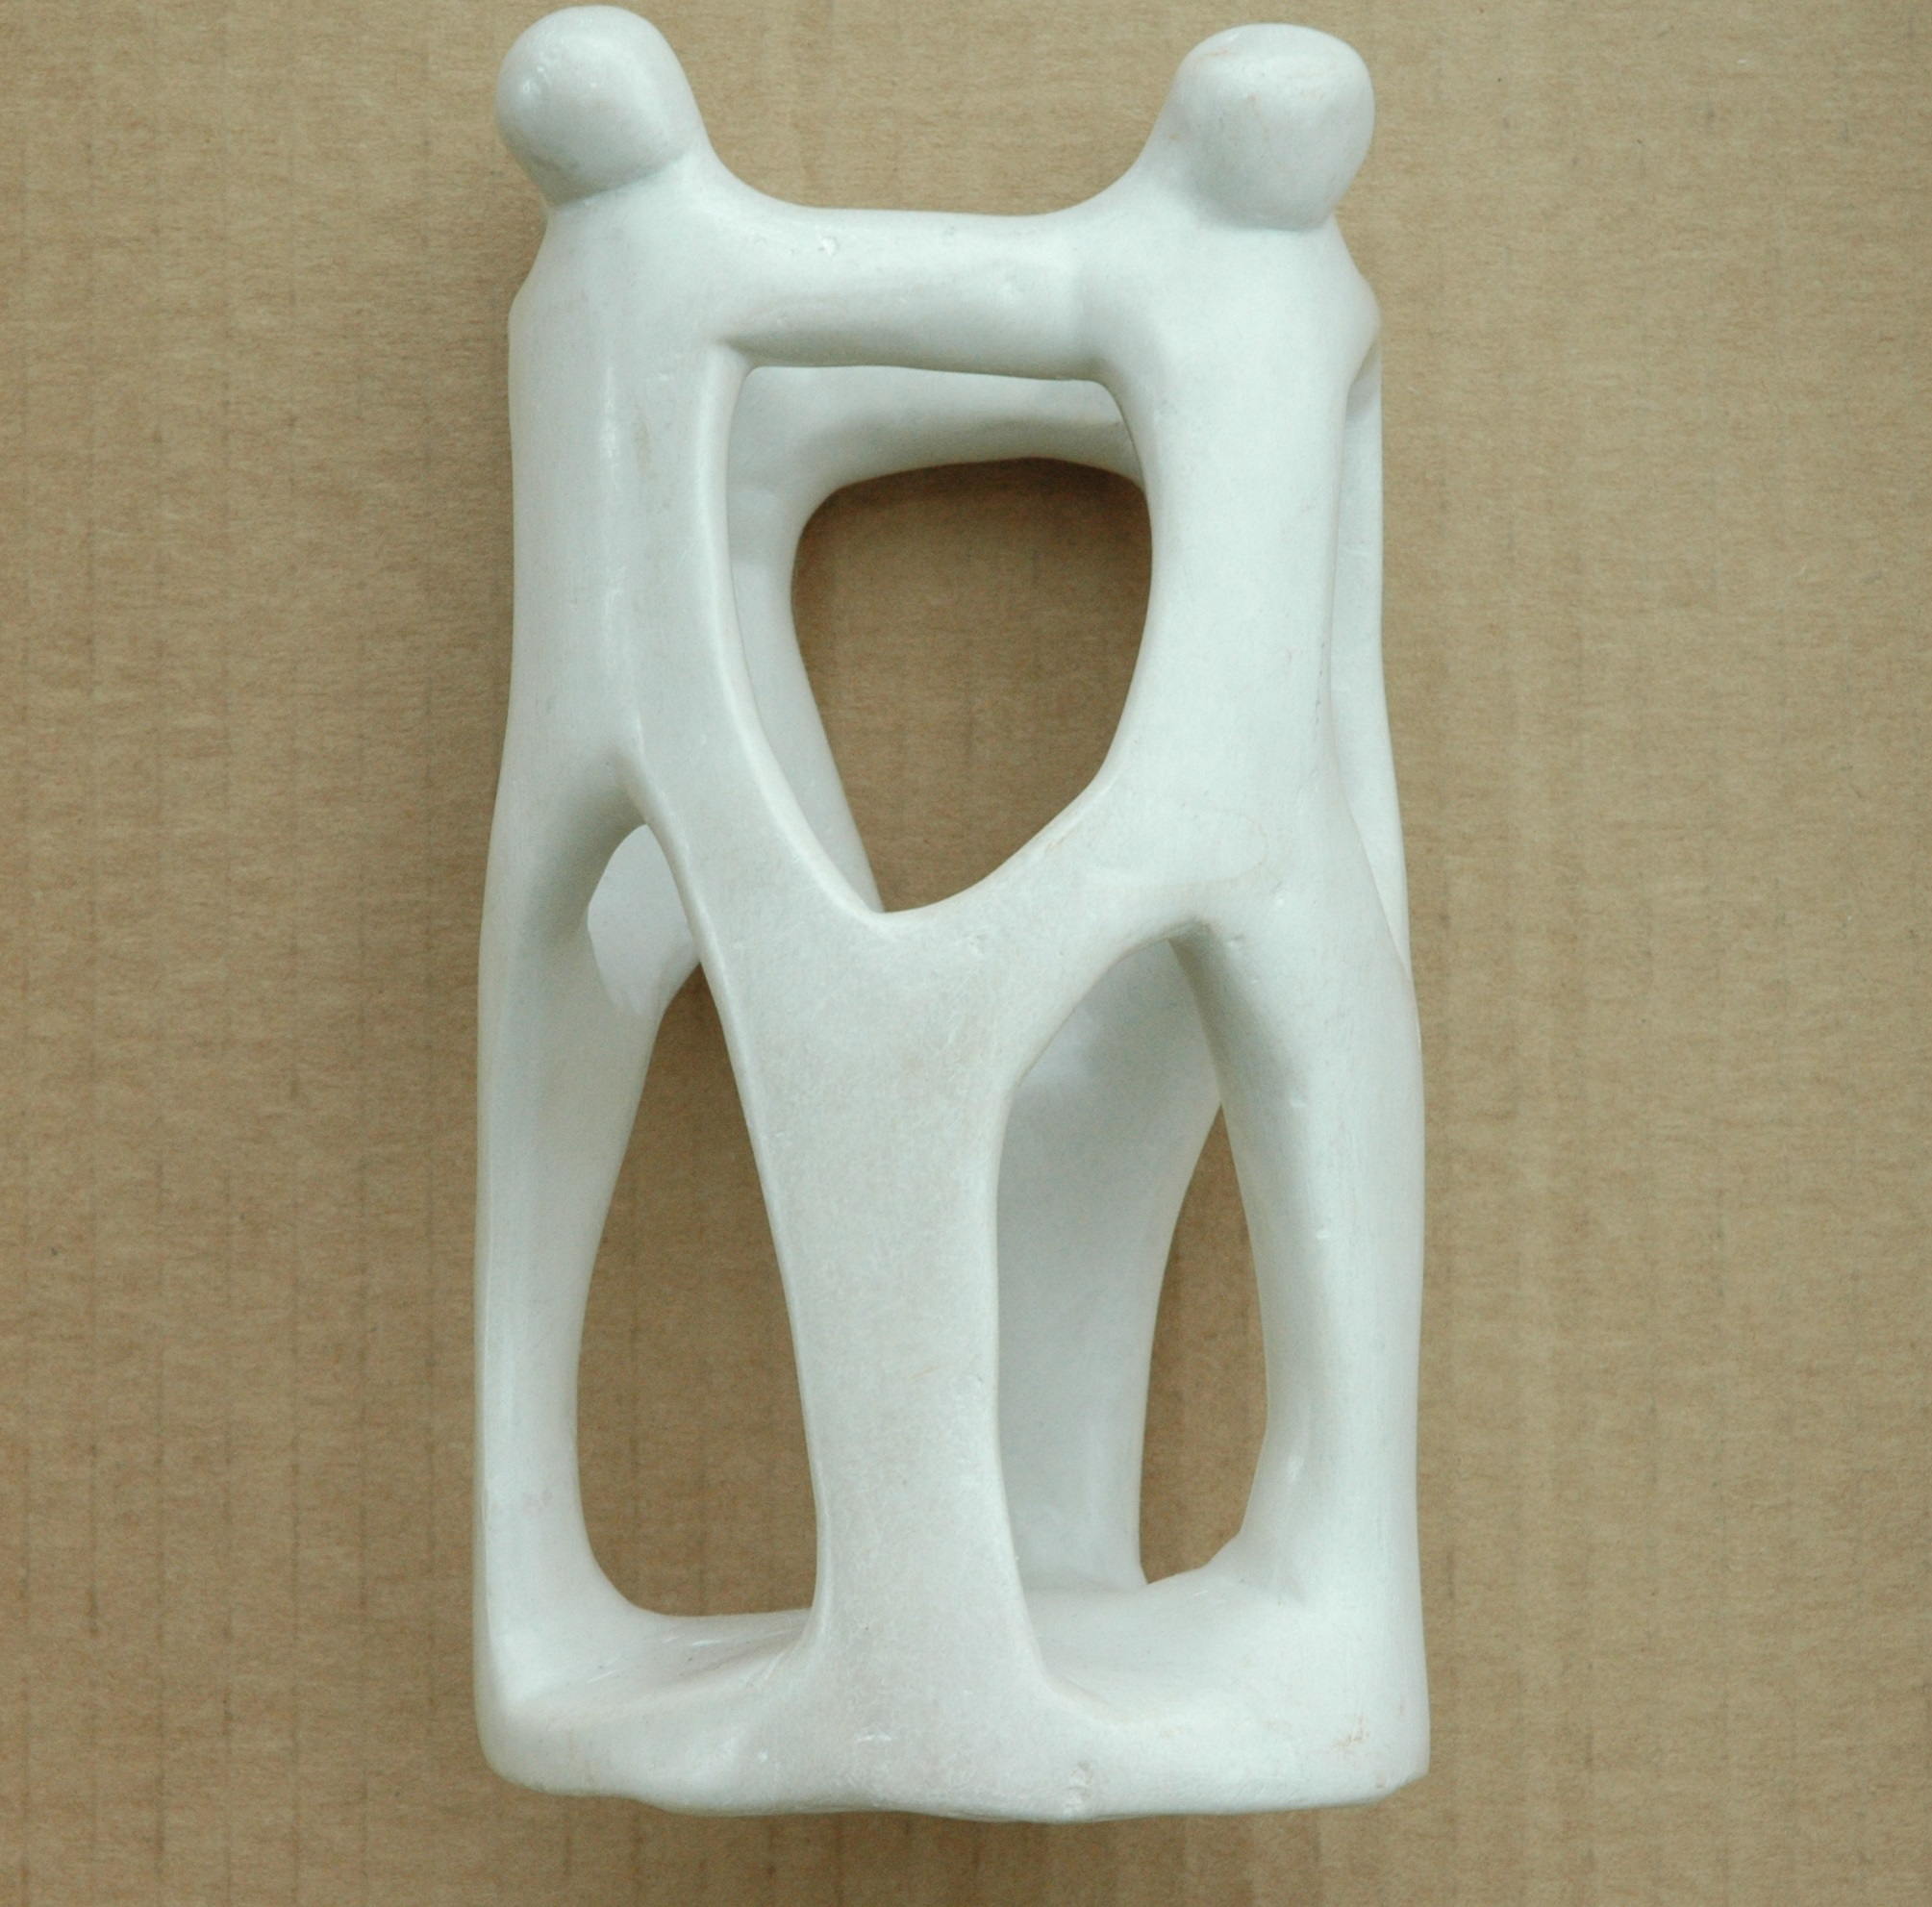
\includegraphics[width=0.15\textwidth]{interp/real_world_img/statue/statue} &
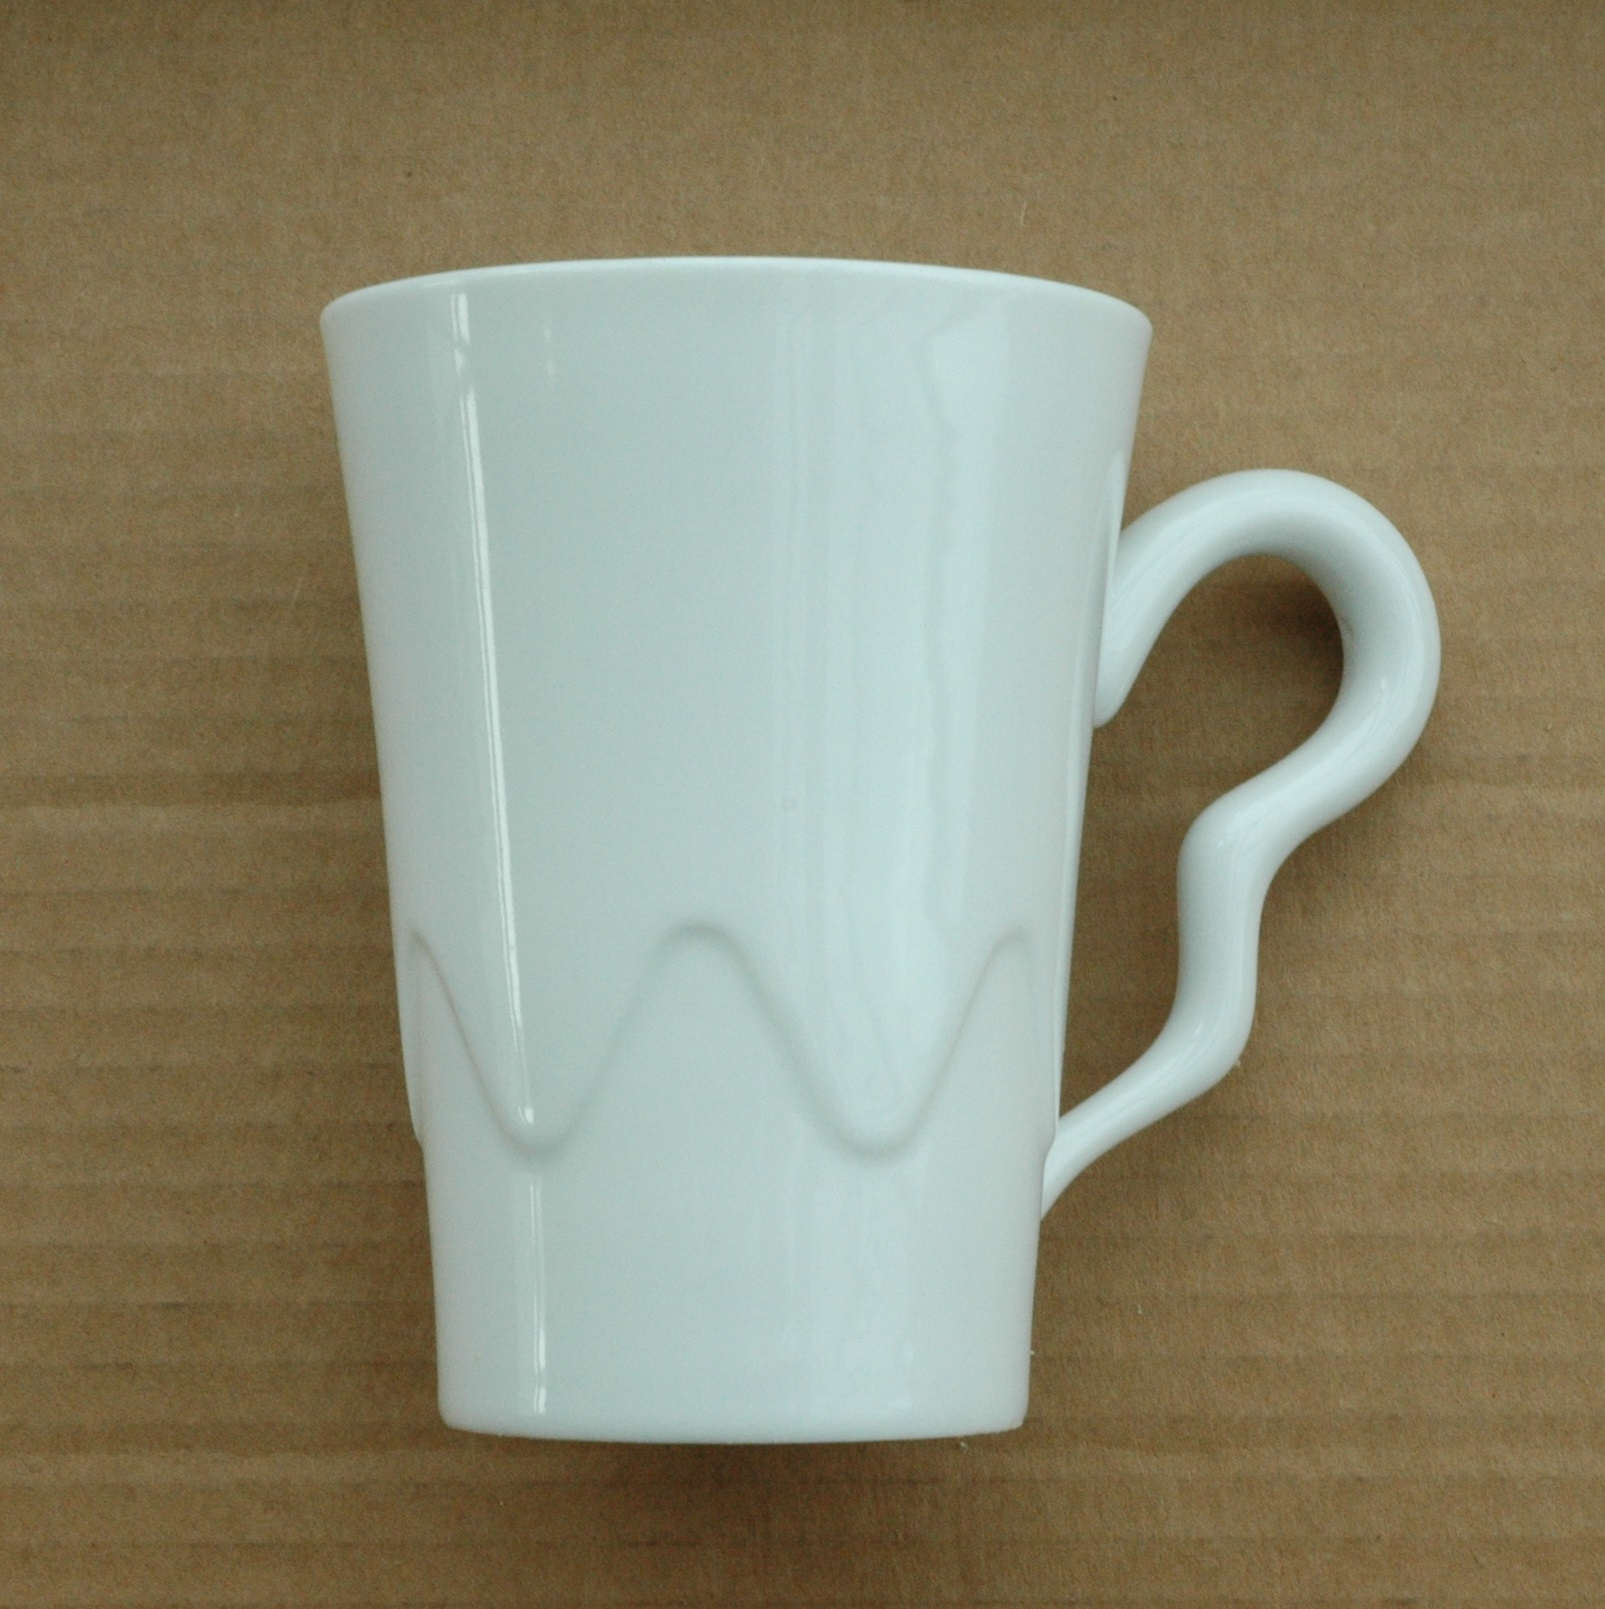
\includegraphics[width=0.15\textwidth]{interp/real_world_img/cup/cup} &
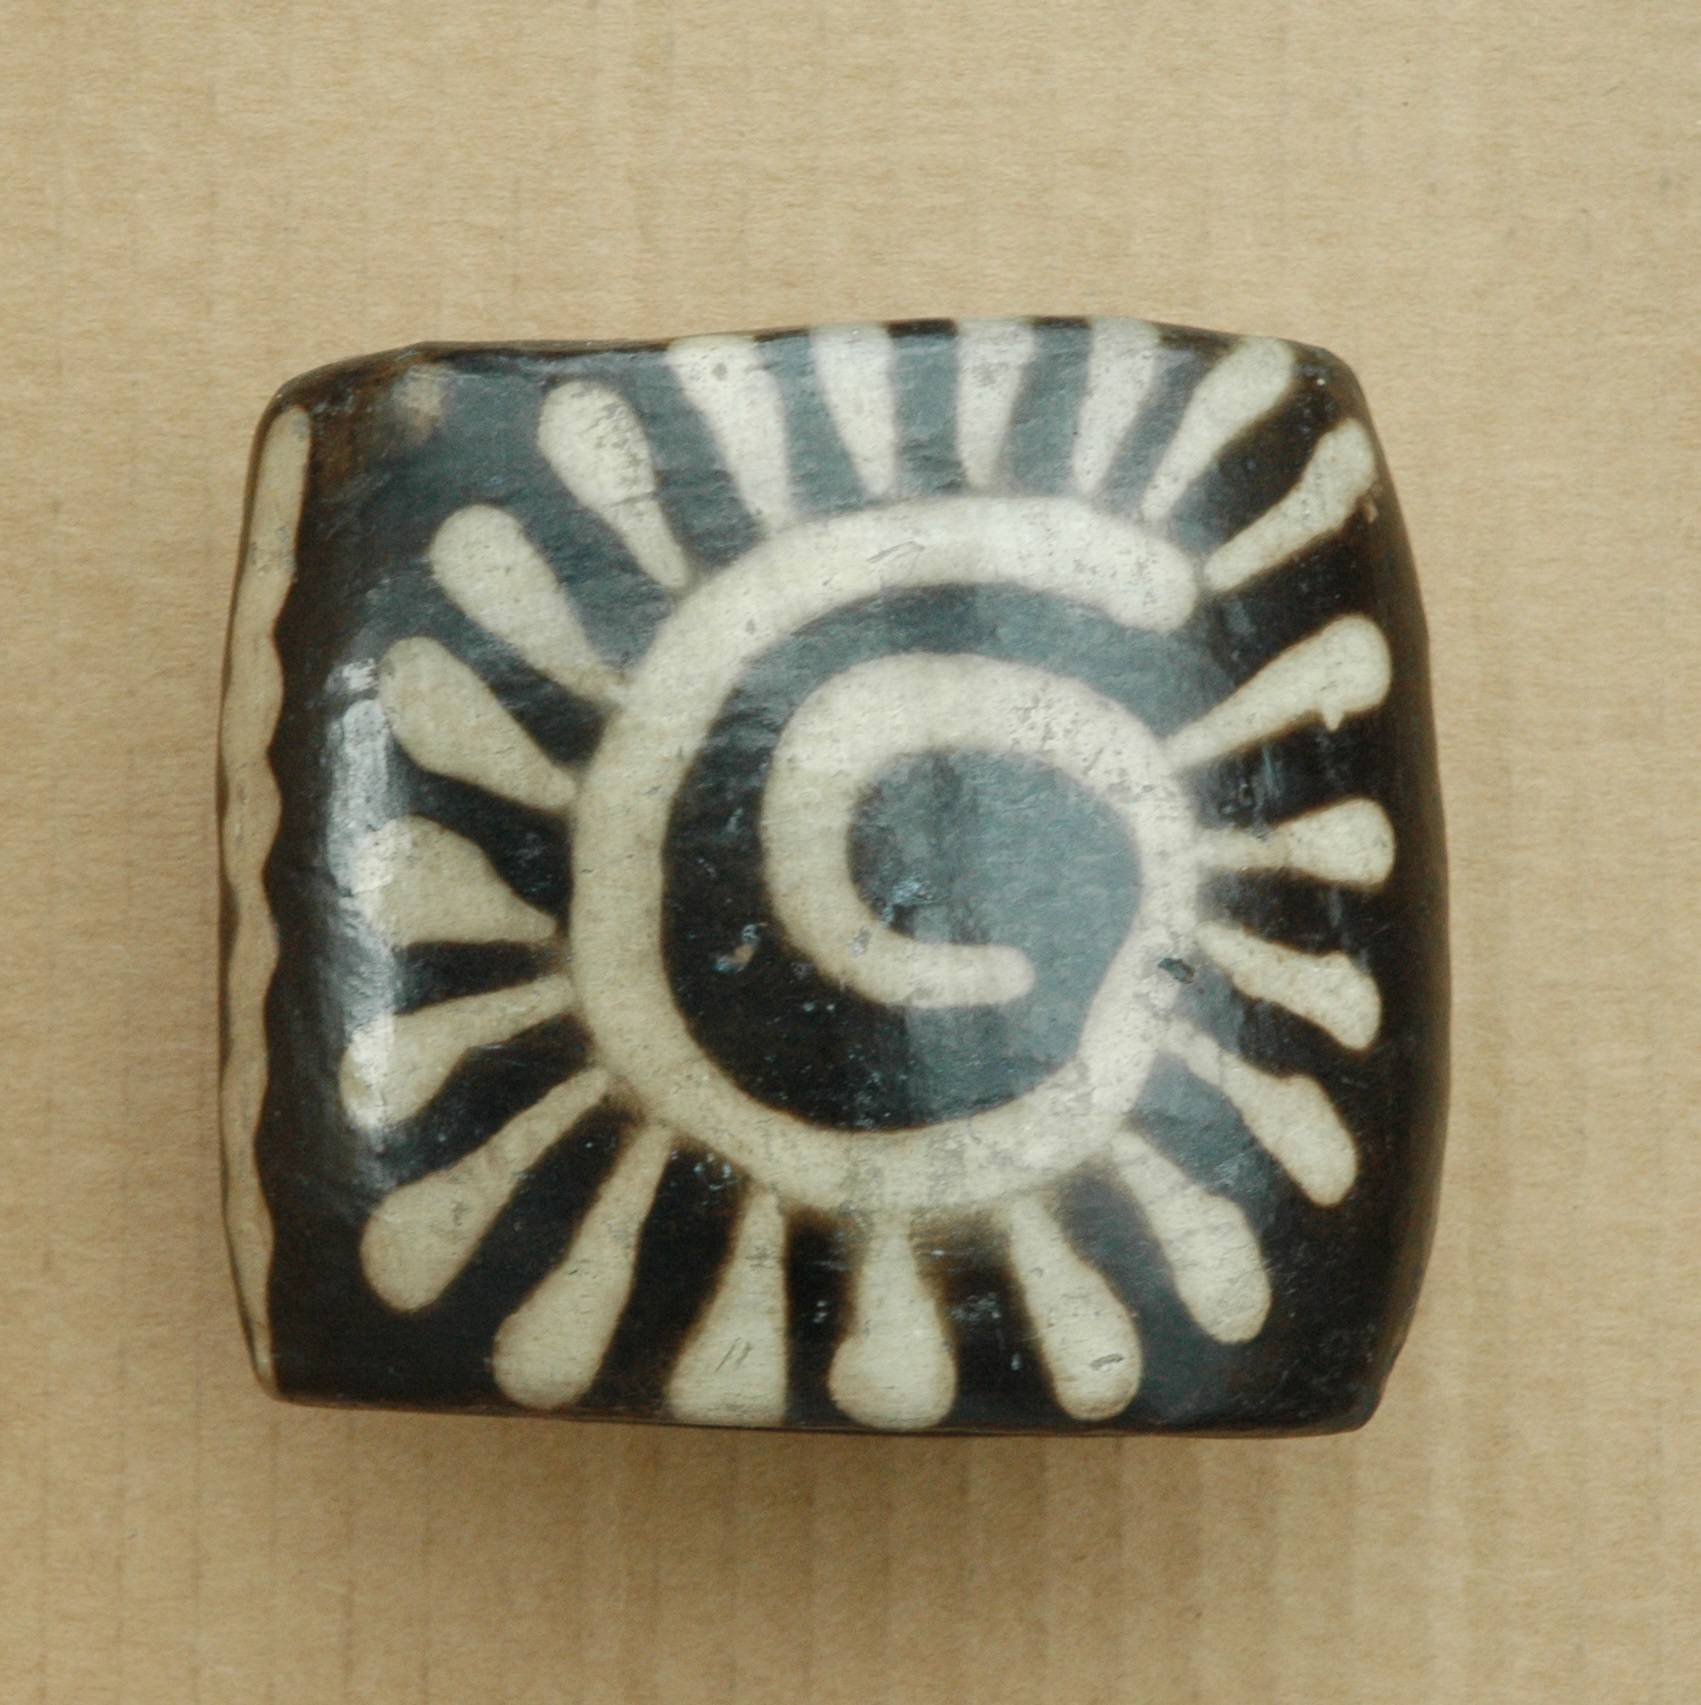
\includegraphics[width=0.15\textwidth]{interp/real_world_img/pot/pot} &
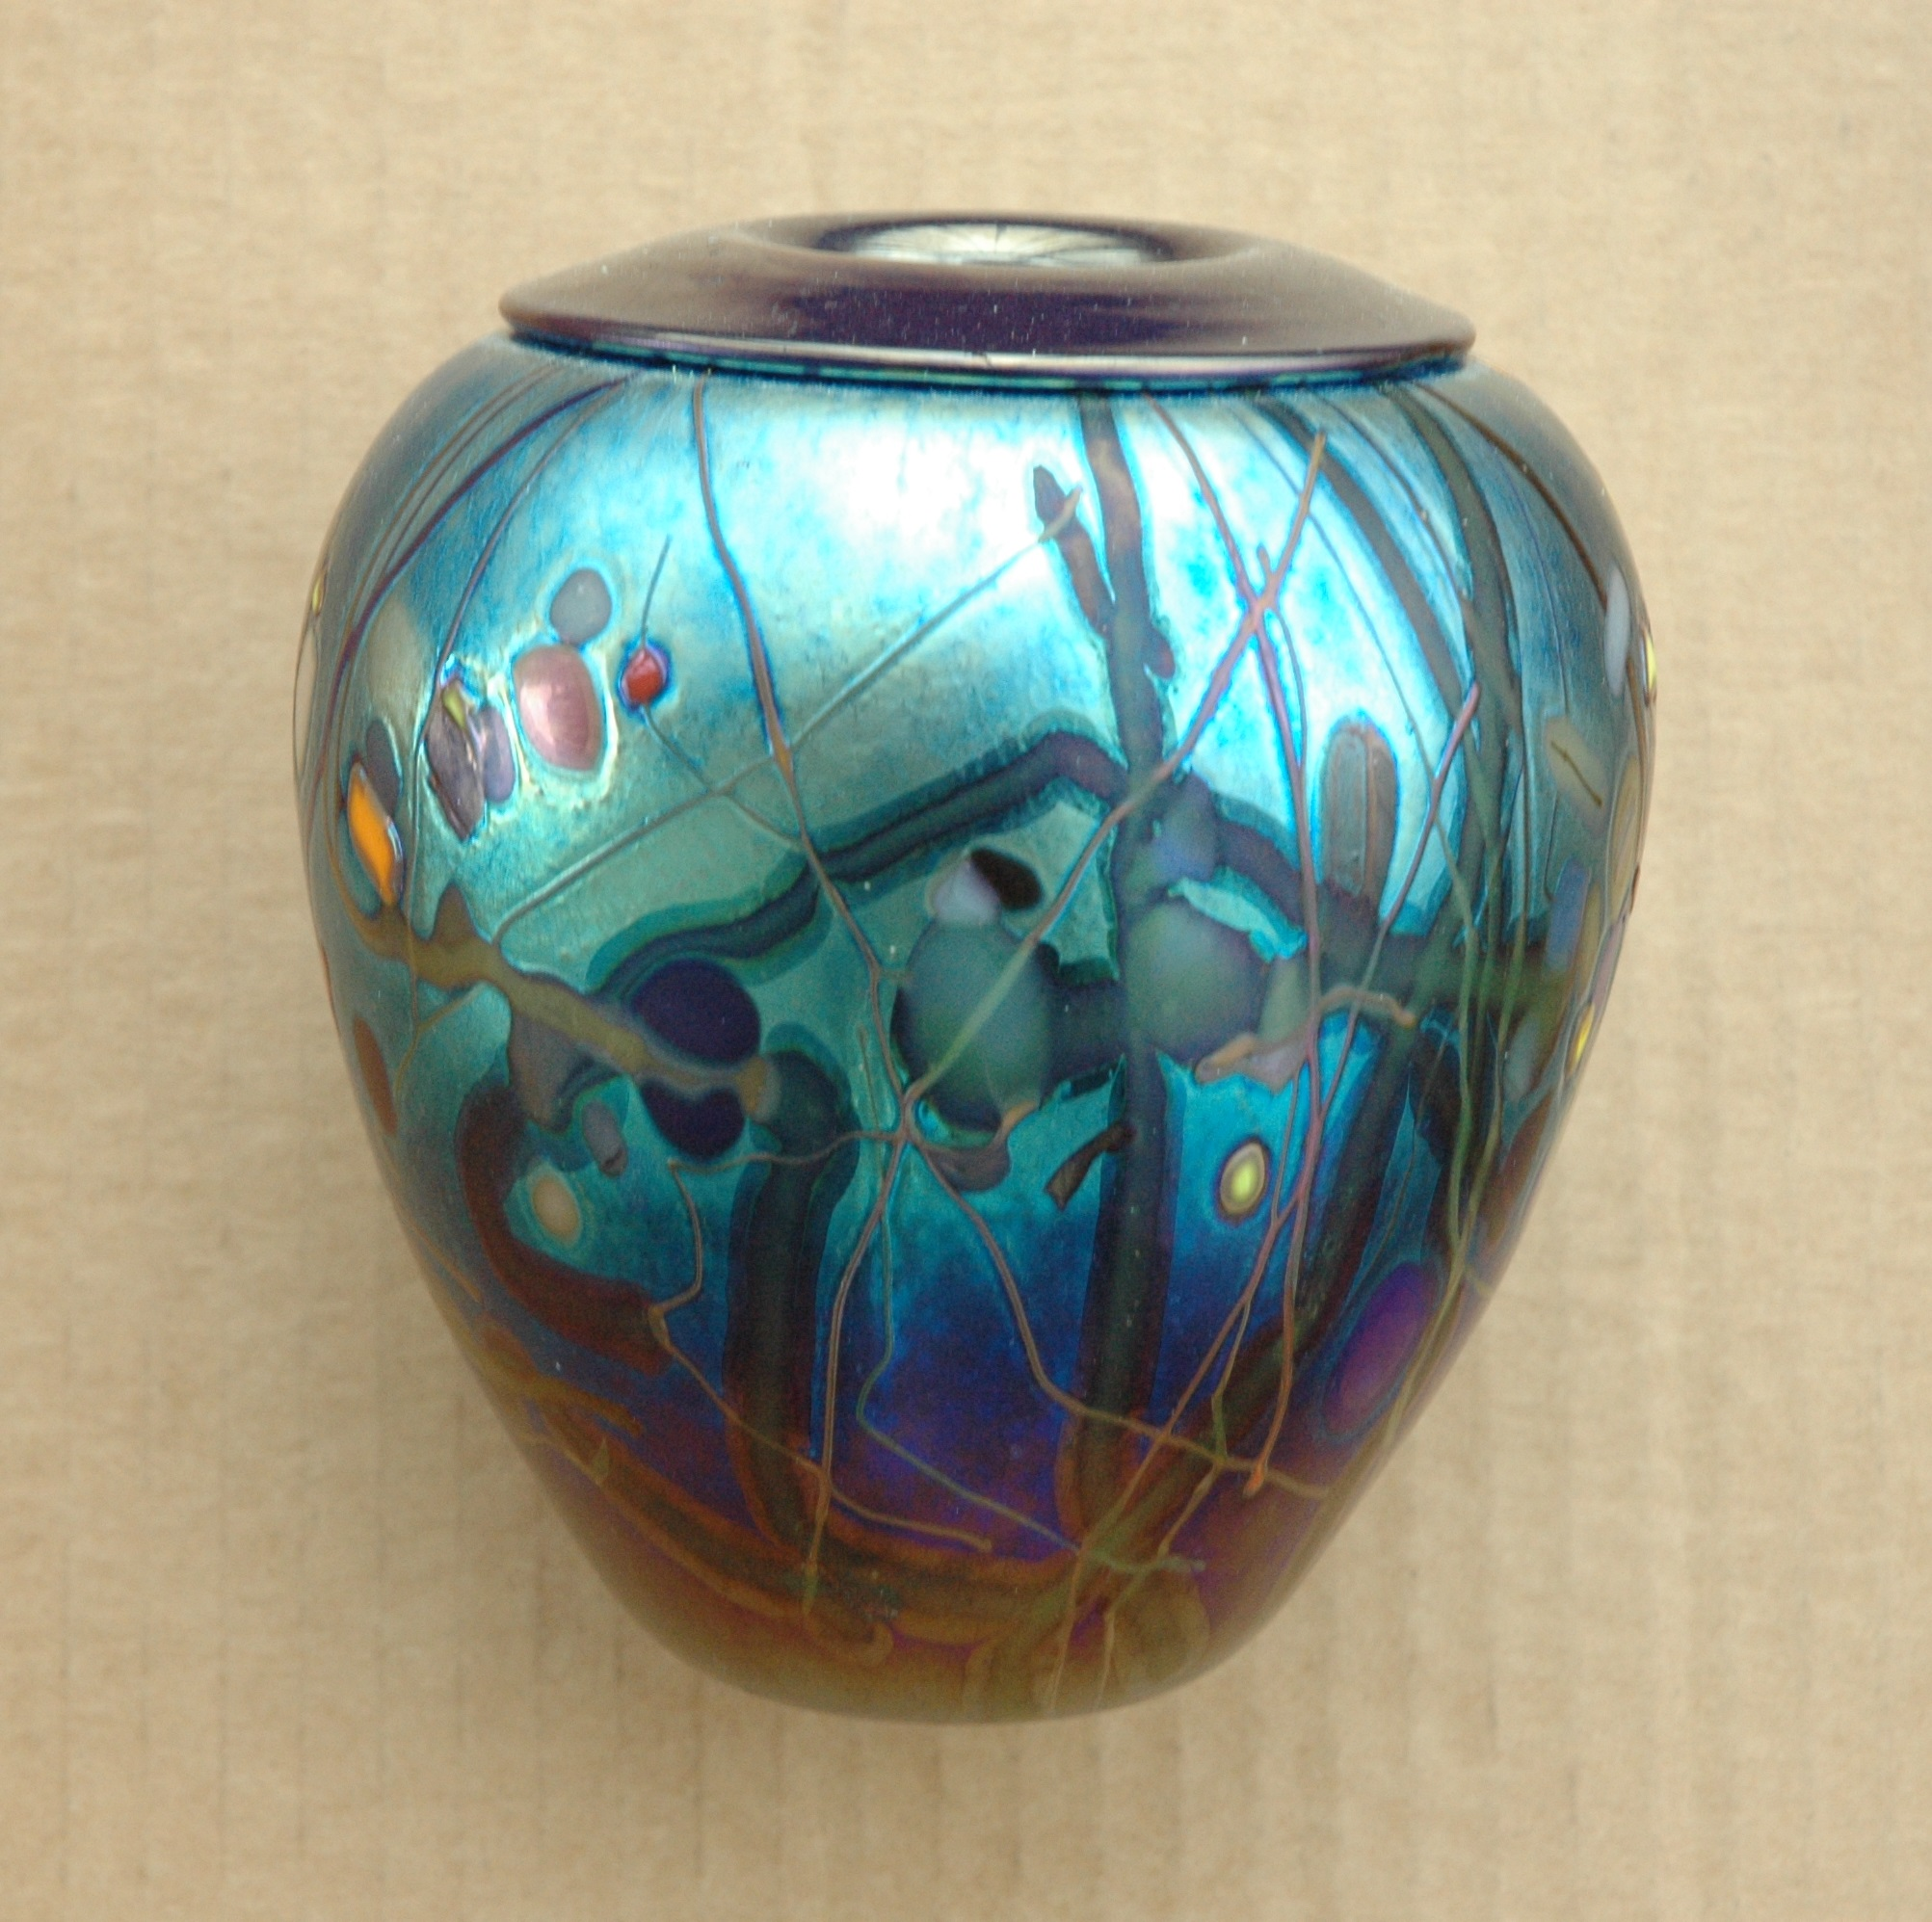
\includegraphics[width=0.15\textwidth]{interp/real_world_img/vase/vase}
% \\ \cline{1-5}
% \multirow{3}{*}{\rotatebox[origin=c]{90}{appearance}}
%   & textureless & textureless & textured & textured\\
%   & diffuse & mixed d/s & diffuse & mixed d/s\\
%   & bright & bright & bright/dark & bright/dark\\
\end{tabular}
\end{figure}

\end{frame}

%------------------------------------------------
\begin{frame}{Interpretation: accurate description, successful result}

\addtolength{\tabcolsep}{-3pt}
\begin{figure}
\centering
\begin{tabular}{*{8}{p{1cm}}}

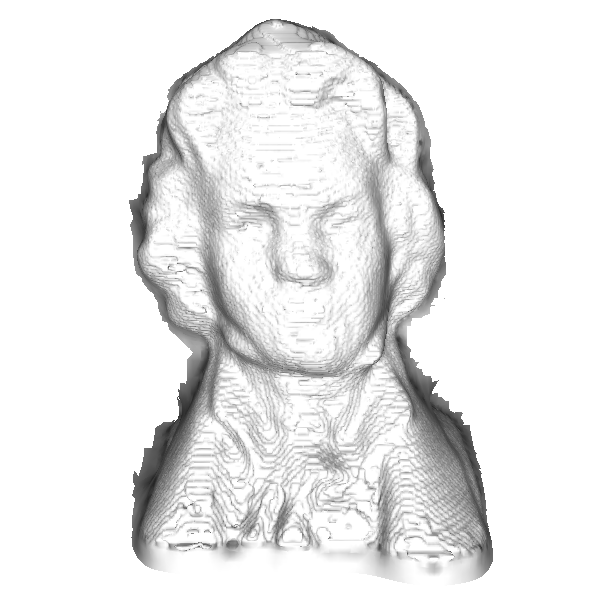
\includegraphics[width=0.12\textwidth]{interp/synth_interp/beethoven_sl} & 
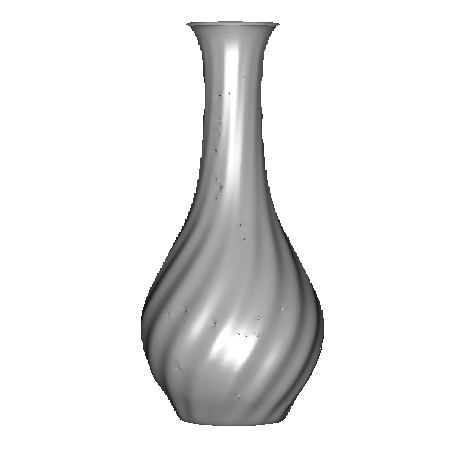
\includegraphics[width=0.12\textwidth]{interp/synth_interp/vase0_ps} &
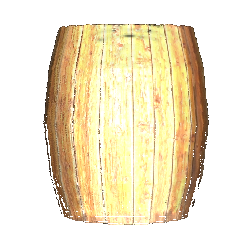
\includegraphics[width=0.12\textwidth]{interp/synth_interp/barrel_sl} &
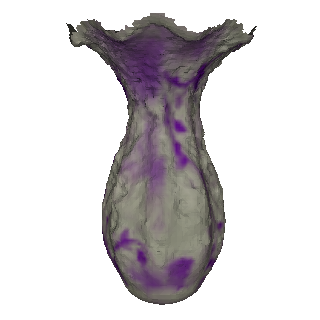
\includegraphics[width=0.12\textwidth]{interp/synth_interp/vase1_mvs} & 
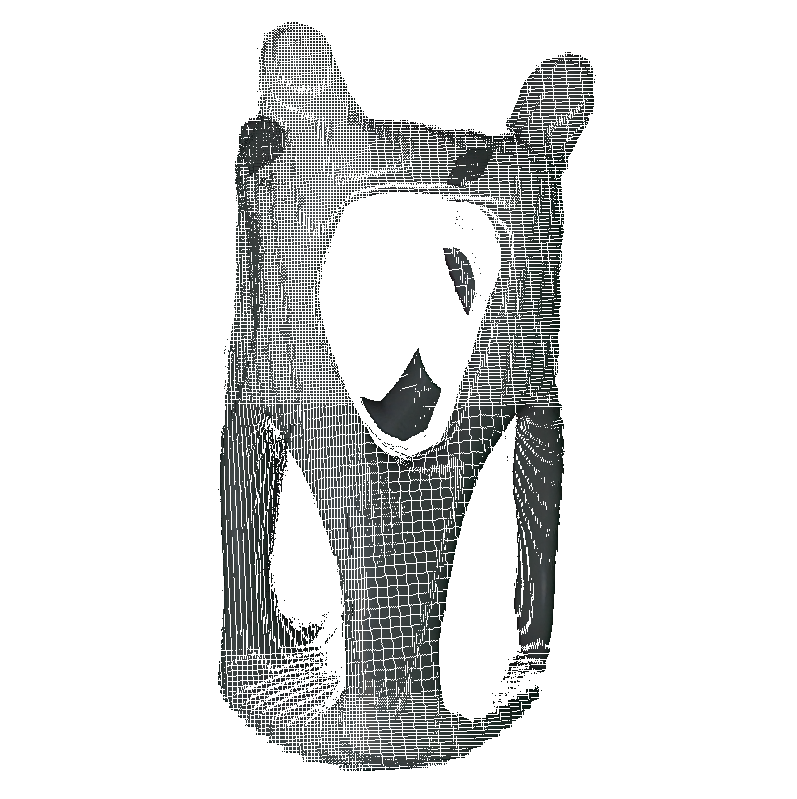
\includegraphics[width=0.12\textwidth]{interp/real_interp/statue/statue_sl} &
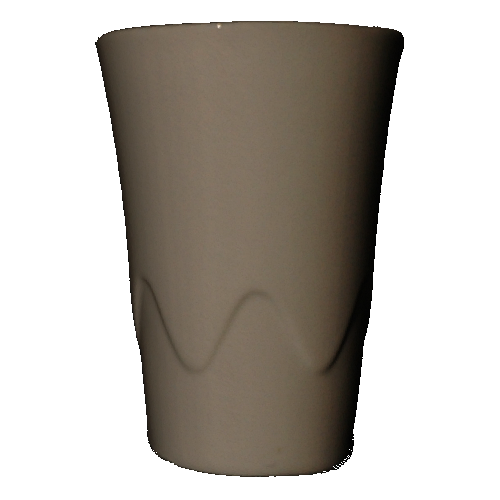
\includegraphics[width=0.12\textwidth]{interp/real_interp/cup/cup_ps} &
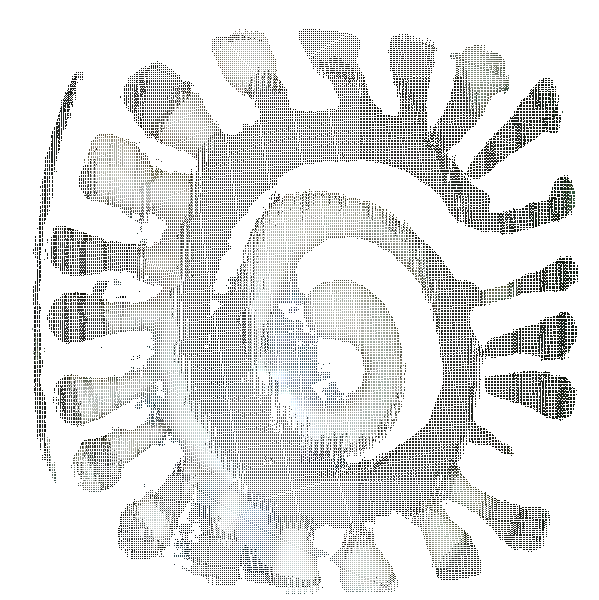
\includegraphics[width=0.12\textwidth]{interp/real_interp/pot/pot_sl} &
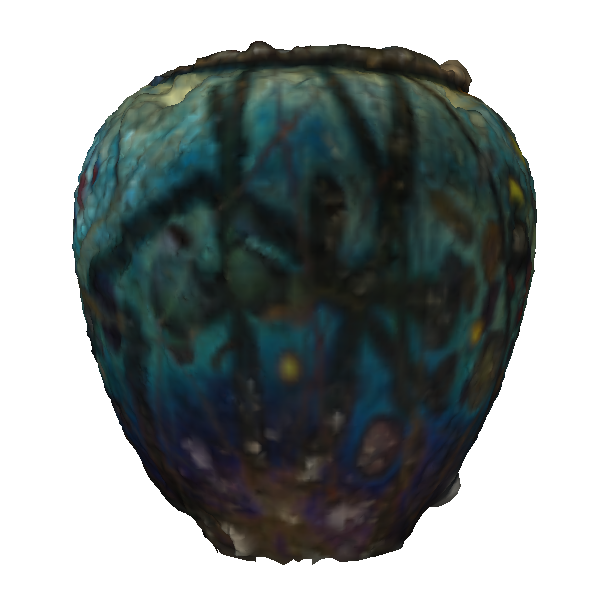
\includegraphics[width=0.12\textwidth]{interp/real_interp/vase/vase_mvs} \\
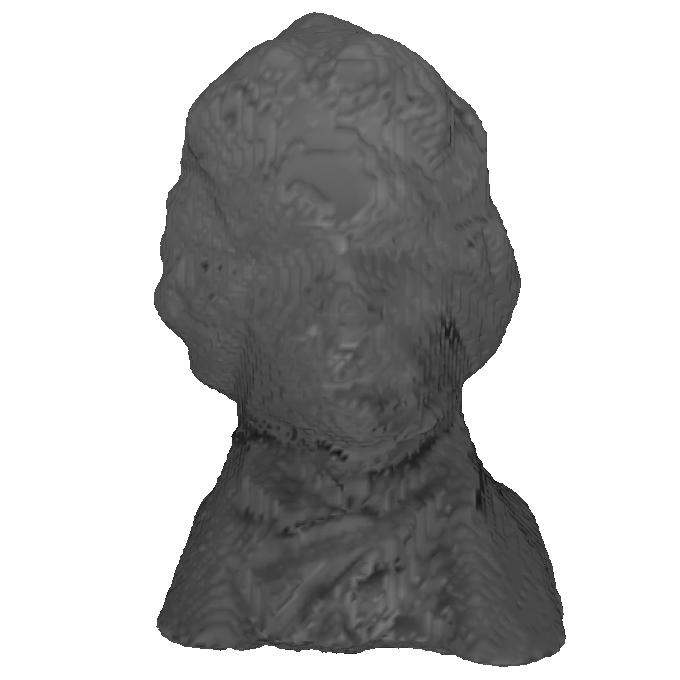
\includegraphics[width=0.12\textwidth]{interp/synth_interp/beethoven_vh} &
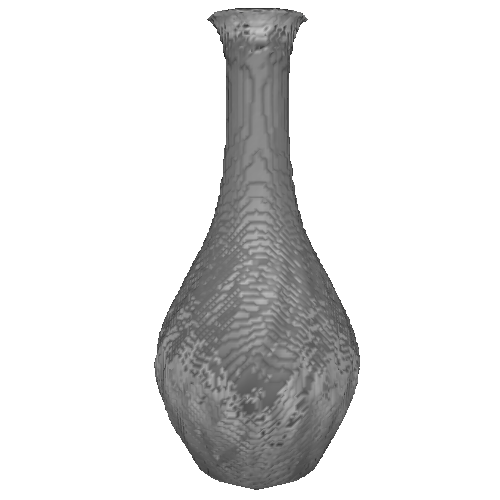
\includegraphics[width=0.12\textwidth]{interp/synth_interp/vase0_vh} &
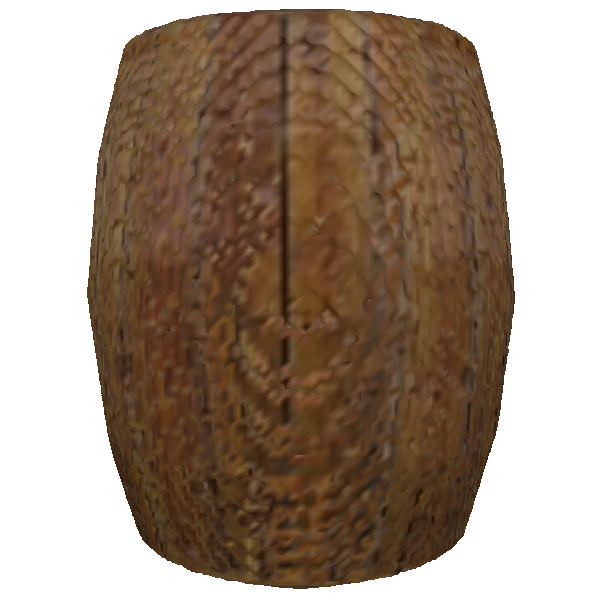
\includegraphics[width=0.12\textwidth]{interp/synth_interp/barrel_vh} &
\includegraphics[width=0.12\textwidth]{interp/synth_interp/vase1_vh} &
\includegraphics[width=0.12\textwidth]{interp/real_interp/statue/statue_sc} &
\includegraphics[width=0.12\textwidth]{interp/real_interp/cup/cup_sc} &
\includegraphics[width=0.12\textwidth]{interp/real_interp/pot/pot_sc} &
\includegraphics[width=0.12\textwidth]{interp/real_interp/vase/vase_sc} \\

\end{tabular}
\end{figure}
\addtolength{\tabcolsep}{3pt}

\begin{exampleblock}{}
\begin{itemize}
\item accuracy: smoother surface, higher quality
\item completenss: no surface holes
\end{itemize}
\end{exampleblock}

\end{frame}

%------------------------------------------------
\begin{frame}{Interpretation: less accurate description, less successful result}

\addtolength{\tabcolsep}{-6pt}
\begin{figure}
\centering
\begin{tabular}{*{5}{c}|*{5}{c}}
\tc{T}ASR & T\tc{A}SR & TA\tc{S}R & TAS\tc{R} & TASR & \tc{T}ASR & T\tc{A}SR & TA\tc{S}R & TAS\tc{R} & TASR \\
\midrule
\includegraphics[width=0.1\textwidth]{interp/synth_interp/vase0_mvs} &
\includegraphics[width=0.1\textwidth]{interp/synth_interp/vase0_vh} &
\includegraphics[width=0.1\textwidth]{interp/synth_interp/vase0_sl} &
\includegraphics[width=0.1\textwidth]{interp/synth_interp/vase0_sl} &
\includegraphics[width=0.1\textwidth]{interp/synth_interp/vase0_ps} &
\includegraphics[width=0.1\textwidth]{interp/real_interp/cup/cup_mvs} &
\includegraphics[width=0.1\textwidth]{interp/real_interp/cup/cup_sc} &
\includegraphics[width=0.1\textwidth]{interp/real_interp/cup/cup_sl} &
\includegraphics[width=0.1\textwidth]{interp/real_interp/cup/cup_sl} &
\includegraphics[width=0.1\textwidth]{interp/real_interp/cup/cup_ps} \\

\includegraphics[width=0.1\textwidth]{interp/synth_interp/vase1_ps} &
\includegraphics[width=0.1\textwidth]{interp/synth_interp/vase1_vh} &
\includegraphics[width=0.1\textwidth]{interp/synth_interp/vase1_sl} &
\includegraphics[width=0.1\textwidth]{interp/synth_interp/vase1_sl} &
\includegraphics[width=0.1\textwidth]{interp/synth_interp/vase1_mvs} &
\includegraphics[width=0.1\textwidth]{interp/real_interp/vase/vase_ps} &
\includegraphics[width=0.1\textwidth]{interp/real_interp/vase/vase_sc} &
\includegraphics[width=0.1\textwidth]{interp/real_interp/vase/vase_sl} &
\includegraphics[width=0.1\textwidth]{interp/real_interp/vase/vase_sl} &
\includegraphics[width=0.1\textwidth]{interp/real_interp/vase/vase_mvs}\\

\end{tabular}
\end{figure}
\addtolength{\tabcolsep}{6pt}

\begin{exampleblock}{}
\begin{itemize}
\item accuracy or completeness: poorer, rougher, incomplete surface.
\end{itemize}
\end{exampleblock}

\end{frame}

%------------------------------------------------
\begin{frame}{Interpretation: less accurate description, less successful result (cont'd)}

\addtolength{\tabcolsep}{-6pt}
\begin{figure}
\centering
\begin{tabular}{*{5}{c}|*{5}{c}}
\tc{T}ASR & T\tc{A}SR & TA\tc{S}R & TAS\tc{R} & TASR & \tc{T}ASR & T\tc{A}SR & TA\tc{S}R & TAS\tc{R} & TASR\\
\midrule

\includegraphics[width=0.1\textwidth]{interp/synth_interp/beethoven_sl} &
\includegraphics[width=0.1\textwidth]{interp/synth_interp/beethoven_ps} &
\includegraphics[width=0.1\textwidth]{interp/synth_interp/beethoven_sl} &
\includegraphics[width=0.1\textwidth]{interp/synth_interp/beethoven_sl} &
\includegraphics[width=0.1\textwidth]{interp/synth_interp/beethoven_sl} &
\includegraphics[width=0.1\textwidth]{interp/real_interp/statue/statue_sl} &
\includegraphics[width=0.1\textwidth]{interp/real_interp/statue/statue_ps} &
\includegraphics[width=0.1\textwidth]{interp/real_interp/statue/statue_sl} &
\includegraphics[width=0.1\textwidth]{interp/real_interp/statue/statue_sl} &
\includegraphics[width=0.1\textwidth]{interp/real_interp/statue/statue_sl} \\

\includegraphics[width=0.1\textwidth]{interp/synth_interp/barrel_sl} &
\includegraphics[width=0.1\textwidth]{interp/synth_interp/barrel_mvs} &
\includegraphics[width=0.1\textwidth]{interp/synth_interp/barrel_sl} &
\includegraphics[width=0.1\textwidth]{interp/synth_interp/barrel_sl} &
\includegraphics[width=0.1\textwidth]{interp/synth_interp/barrel_sl} &
\includegraphics[width=0.1\textwidth]{interp/real_interp/pot/pot_sl} &
\includegraphics[width=0.1\textwidth]{interp/real_interp/pot/pot_mvs} &
\includegraphics[width=0.1\textwidth]{interp/real_interp/pot/pot_sl} &
\includegraphics[width=0.1\textwidth]{interp/real_interp/pot/pot_sl} &
\includegraphics[width=0.1\textwidth]{interp/real_interp/pot/pot_sl} \\

\end{tabular}
\end{figure}
\addtolength{\tabcolsep}{6pt}

\begin{exampleblock}{}
\begin{itemize}
\item accuracy or completeness: comparable 
\item less accurate descriptions trigger the same algorithm as the accurate one.
\end{itemize}
\end{exampleblock}

\end{frame}

%------------------------------------------------
\begin{frame}{Interpretation: inaccurate description, poor result}

\addtolength{\tabcolsep}{-3pt}
\begin{figure}
\centering
\begin{tabular}{*{8}{p{1cm}}}

\includegraphics[width=0.12\textwidth]{interp/synth_interp/beethoven_vh} &
\includegraphics[width=0.12\textwidth]{interp/synth_interp/vase0_mvs} &
\includegraphics[width=0.12\textwidth]{interp/synth_interp/barrel_vh} &
\includegraphics[width=0.12\textwidth]{interp/synth_interp/vase1_ps} &
\includegraphics[width=0.12\textwidth]{interp/real_interp/statue/statue_sc} &
\includegraphics[width=0.12\textwidth]{interp/real_interp/cup/cup_mvs} &
\includegraphics[width=0.12\textwidth]{interp/real_interp/pot/pot_sc} &
\includegraphics[width=0.12\textwidth]{interp/real_interp/vase/vase_ps} \\

\includegraphics[width=0.12\textwidth]{interp/synth_interp/beethoven_sl} &
\includegraphics[width=0.12\textwidth]{interp/synth_interp/vase0_ps} &
\includegraphics[width=0.12\textwidth]{interp/synth_interp/barrel_sl} &
\includegraphics[width=0.12\textwidth]{interp/synth_interp/vase1_mvs} &
\includegraphics[width=0.12\textwidth]{interp/real_interp/statue/statue_sl} &
\includegraphics[width=0.12\textwidth]{interp/real_interp/cup/cup_ps} &
\includegraphics[width=0.12\textwidth]{interp/real_interp/pot/pot_sl} &
\includegraphics[width=0.12\textwidth]{interp/real_interp/vase/vase_mvs} \\

\end{tabular}
\end{figure}
\addtolength{\tabcolsep}{3pt}

\begin{exampleblock}{}
\begin{itemize}
\item Baseline method is selected by the interface;
\item accuracy or completeness: poor, rougher, incomplete surface.
\end{itemize}
\end{exampleblock}

\end{frame}

%------------------------------------------------
\begin{frame}{Interpretation: discussions}

\begin{exampleblock}{}
\begin{itemize}
\item We have demonstrated that it is achievable to design an description-based interface so that a successful reconstruction result is obtained given a description of problem condition, without knowledge of which algorithm to use;
\item Algorithm chosen by the interpreter given a less accurate description may or may not achieve a poor result;
\item Algorithm chosen by the interpreter given inaccurate description is more likely to achieve a poorer result.
% \item It depends if the return algorithms has at least an overlapping with those returned if given accurate description;
% \item The reconstruction result becomes worse as the description becomes less accurate.
\end{itemize}
\end{exampleblock}

\end{frame}

%------------------------------------------------
\begin{frame}{Interpreter: summary}

\begin{figure}
\centering
\includegraphics[width=0.9\textwidth]{images/3d_recon_interface_2.pdf}
\end{figure}

\begin{exampleblock}{}
  \begin{itemize}
    \item \textbf{Algorithms}: description of appearance, no vision background needed, embeding new algorithms is easy;
    \item \textbf{Parameters}: property parameters are perceptually interpretable\& meaningful;
    \item \textbf{Approach}: no \textit{trial-and-error}.
  \end{itemize}
\end{exampleblock}

\end{frame}

%------------------------------------------------
\section{Conclusions}
%------------------------------------------------
\begin{frame}{Conclusions}

\begin{exampleblock}{}

\begin{itemize}
\item The proposed interface is able to produce a correct reconstruction result given an accurate description of an object;
\item The solution produced by the interface improves as the description becomes more accurate;
\item Using the description and proof of concept interpreter, we demonstrate the possibility of using descriptive properties to hide algorithm details and providing a fixed set of parameters that can be perceptually estimated.
\end{itemize}

\end{exampleblock}

\end{frame}

%------------------------------------------------
\begin{frame}{Future directions}

\begin{exampleblock}{}

\begin{itemize}
\item Develop automated approach to derive description from images;
\item Develop more advanced techniques to discover the mapping from problem conditions to algorithms;
\item Develop more sophisticated geometric model to incorporate objects with complex geometry.
\item Investigate the more precise relation between description and performance, \emph{i.e.,} if better description can lead to better performance monotonically.
% \item To deal with more complicated objects, we need more complicated properties, or ways to describe the objects, but the challenge is the easy mathematical representation might not be available.
\end{itemize}

\end{exampleblock}

\end{frame}

%------------------------------------------------
\begin{frame}[standout]

Computer vision should focus on more than \\just algorithms, but easier accessibility.

\end{frame}

%------------------------------------------------
% Additional material
%------------------------------------------------
\appendix
\begin{frame}{Description: expression}

We use three-scale values to parameterize properties: \textit{low} (0.2), \textit{medium} (0.5), and \textit{high} (0.8).

\begin{figure}[!htbp]
\centering
\begin{tabular}{cccc}
  \includegraphics[width=0.25\textwidth]{images/desc_vase.pdf}&
  \includegraphics[width=0.2\textwidth]{interp/ui/ui_sphere.png}&
  \includegraphics[width=0.2\textwidth]{interp/ui/ui_vase.png}&
  \includegraphics[width=0.2\textwidth]{interp/real_world_img/vase/vase.jpg}\\
  Property settings & Synthetic sphere & Synthetic vase & Real-world vase\\
\end{tabular}
% \caption{(a) demonstrates the effect of the property settings on a sphere, (b) on a teapot, and (c) shows the real-world object.}
\end{figure}

\end{frame}

%------------------------------------------------
\begin{frame}{Mapping: algorithms}

\begin{exampleblock}{selected algorithms}
\begin{itemize}
\item Patch-based Multi-View Stereo (PMVS): propagate-refinement-filtering;
\item Example-based Photometric Stereo (EPS): arbitrary BRDF is a linear combination of basis BRDFs;
\item Gray-coded Structured Light (GSL): encode spatial informally temporally.
\end{itemize}
\end{exampleblock}

\begin{exampleblock}{baseline methods}
\begin{itemize}
\item Volumetric Visual Hull: carve voxels projecting outside of silhouettes;
\item Linear-least squares Photometric Stereo: $\mathbf{I}=\rho\mathbf{N}\cdot\mathbf{L}$
\end{itemize}
\end{exampleblock}

\end{frame}

%------------------------------------------------
\begin{frame}{Mapping: interesting observations}

% We provide key observations that can be theoretically justified by theory to demonstrate the insights that could be obtained from the mapping.

\begin{exampleblock}{1. PMVS can work on specular surfaces provided the surface highly textured}
\begin{figure}
\begin{tabular}{ccc}
\includegraphics[width=0.22\textwidth]{mapping/mvs_spec/mvs_spec}&
\includegraphics[width=0.22\textwidth]{mapping/mvs_spec/mvs_spec_01}&
\includegraphics[width=0.22\textwidth]{mapping/mvs_spec/mvs_spec_00}\\
% (a). Image formation & (b) $V_1$ & (c) $V_2$\\
\end{tabular}
\end{figure}
\end{exampleblock}

\begin{exampleblock}{2. EPS and GSL fails on highly specular surfaces, and a blurred specular area leads to worse results.}
\begin{figure}
\begin{tabular}{ccc}
\includegraphics[width=0.15\textwidth]{mapping/ps_spec_rough/0802_normal}&
\includegraphics[width=0.15\textwidth]{mapping/ps_spec_rough/0805_normal}&
\includegraphics[width=0.15\textwidth]{mapping/ps_spec_rough/0808_normal}\\
(a). rough: 0.2 & (b). rough: 0.5 & (c). rough: 0.8
\end{tabular}
\end{figure}
\end{exampleblock}

\end{frame}

%------------------------------------------------
% \begin{frame}{Mapping: notable findings 1}

% \begin{figure}[!htbp]
% \begin{tabular}{cc}
% \includegraphics[width=0.22\textwidth]{mapping/pairwise/mvs_tex_spec}&
% \includegraphics[width=0.22\textwidth]{mapping/mvs_spec/mvs_spec}\\
% (a). Algo. performance & (b) Image formation\\
% \includegraphics[width=0.22\textwidth]{mapping/mvs_spec/mvs_spec_01}&
% \includegraphics[width=0.22\textwidth]{mapping/mvs_spec/mvs_spec_00}\\
% (c) $V_1$ & (d) $V_2$\\
% \end{tabular}
% \caption{(a) shows the algorithm performance w.r.t. texture and specularity. (b) shows the reflection of light off a specular surface. $V_1$ received the diffuse component while $V_2$ receives the specular component. (c), (d) shows the images observed from these two views. The specular area (red circle) observed in $V_2$ is visible in $V_1$.}
% \end{figure}

% \end{frame}

%------------------------------------------------
% \begin{frame}{Mapping: notable findings 2}

% \begin{figure}[!htbp]
% \centering
% \begin{tabular}{c|ccc}
%   Image & Normal map & Height map & Angular error\\
%   \hline\\
%   \includegraphics[width=0.12\textwidth]{mapping/ps_spec_rough/0802_0001}&
%   \includegraphics[width=0.12\textwidth]{mapping/ps_spec_rough/0802_normal}&
%   \includegraphics[width=0.15\textwidth]{images/0802_dmap}&
%   \includegraphics[width=0.05\textwidth]{mapping/ps_spec_rough/0802_ang_error}\\
%   & (a). rough: 0.2\\
%   \includegraphics[width=0.12\textwidth]{mapping/ps_spec_rough/0805_0001}&
%   \includegraphics[width=0.12\textwidth]{mapping/ps_spec_rough/0805_normal}&
%   \includegraphics[width=0.15\textwidth]{images/0805_dmap}&
%   \includegraphics[width=0.05\textwidth]{mapping/ps_spec_rough/0805_ang_error}\\
%   & (b). rough: 0.5\\
%   \includegraphics[width=0.12\textwidth]{mapping/ps_spec_rough/0808_0001}&
%   \includegraphics[width=0.12\textwidth]{mapping/ps_spec_rough/0808_normal}&
%   \includegraphics[width=0.15\textwidth]{images/0808_dmap}&
%   \includegraphics[width=0.05\textwidth]{mapping/ps_spec_rough/0808_ang_error}\\
%   & (c). rough: 0.8\\
% \end{tabular}
% \caption{The effect of roughness on PS. Albedo is set as 0.8, and specular is set as 0.8. (b) demonstrates that a medium level roughness would lead to worse normal estimation since it blurs the specular lobe.}
% \end{figure}

% \end{frame}

%------------------------------------------------
% \begin{frame}{Mapping: notable findings 3}

% \begin{figure}[!htbp]
% \centering
% \begin{tabular}{ccc}
% \includegraphics[width=0.25\textwidth]{trash/mapping/sl_spec_rough/sl_00050202}&
% \includegraphics[width=0.25\textwidth]{trash/mapping/sl_spec_rough/sl_00050502}&
% \includegraphics[width=0.25\textwidth]{trash/mapping/sl_spec_rough/sl_00050802}\\
% (a) specular: 0.2 & (b) specular: 0.5 & (c) specular: 0.8\\
% \includegraphics[width=0.25\textwidth]{trash/mapping/sl_spec_rough/sl_00050802}&
% \includegraphics[width=0.25\textwidth]{trash/mapping/sl_spec_rough/sl_00050805}&
% \includegraphics[width=0.25\textwidth]{trash/mapping/sl_spec_rough/sl_00050808}\\
% (d) roughness: 0.2 & (e) roughness: 0.5 & (f) roughness: 0.8\\
% \end{tabular}
% \caption{(a)-(c): the roughness is set as 0.2, and specular has a negative effect on completeness; (d)-(e): the specular is set as 0.8, roughness has a positive effect on completeness.}
% \end{figure}

% \end{frame}

%------------------------------------------------
\begin{frame}{Interpretation: proof of concept interpreter}

Interpreter: selects an algorithm based on a description.

\begin{figure}[!htbp]
\centering
\includegraphics[width=0.7\textwidth]{interp/interpreter.pdf}
\end{figure}

\end{frame}

%------------------------------------------------
\begin{frame}{Interpretation 2: demonstrative result (cont'd)}

\begin{figure}
\centering
\includegraphics[width=\textwidth]{images/interp2_2.pdf}
\end{figure}

\end{frame}

\end{document}
